\Chapter{Étude de plasmas magnétisés}
\chaptermark{Étude de plasmas magnétisés}
\label{EtudePlasmaMag}
\begin{refsection}
Ce cinquième chapitre porte sur l'étude de trois cas de test simplifiés,
inspirés d'expérimentations réelles. Chacun des cas possède sa problématique
spécifique, et est représentatif d'une configuration magnétique
particulière :

\begin{itemize}
  \item le filtre magnétique avec le propulseur PEGASES
  \item la colonne de plasma magnétisée de la source d'ions négatifs CYBELE
  \item une région de bord de tokamak fortement magnétisée
\end{itemize}

A travers ces exemples, nous testons les possibilités du nouveau code MAGNIS,
tout en explorant la physique qu'il révèle. Les simulations sont discutées et
les phénomènes observés confrontés aux observations expérimentales et
numériques.

\section{Barrière magnétique - PEGASES}
La configuration filtre magnétique utilisée dans PEGASES est caractéristique
dans de nombreuses applications pour diminuer la température électronique

PEGASES, acronyme de \emph{Plasma Propulsion with Electronegative Gases}, est
un prototype de propulseur électrostatique à grille (PEG)
ion-ion~\parencite{Chabert} conçu au LPP (Laboratoire de Physique des
Plasma) de l'École Polytechnique de Paris, et dont l'originalité est d'éjecter
alternativement des ions négatifs et des ions positifs issus d'un plasma ion-ion continu.
Dans ce nouveau concept, les faisceaux d'ions de charges opposées se
neutralisent mutuellement à la sortie du propulseur, ce qui permet de se
libérer de l'utilisation de la cathode neutralisante habituellement requise
pour éviter la polarisation du dispositif.
Pour filtrer les électrons chauds et favoriser la création du plasma ion-ion, une
barrière magnétique d'une centaine de Gauss est placée entre la zone
d'ionisation et la région d'extraction. La structure en différents étages de PEGASES est représentée sur la
figure \ref{4-pegases3D} :

\begin{figure}[!htbp]
\centering
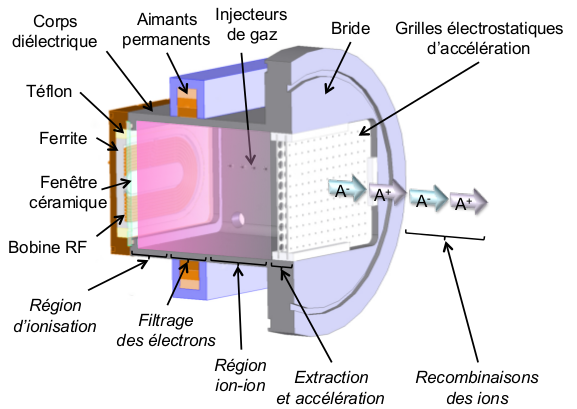
\includegraphics[width=0.75\textwidth]{figures/4-pegases3D.png}
{\caption{Schéma de principe de fonctionnement du propulseur PEGASES avec les
différents étages mentionnés en italiques\parencite{Popelier}.}
\label{4-pegases3D}}
\end{figure}

Dans le premier étage, un gaz électronégatif est
excité inductivement par une puissance RF.
Le plasma de la source, constitué d'ion positifs, d'ions négatifs et d'électrons
est ensuite filtré par une barrière magnétique dans le deuxième étage du
propulseur. L'intensité de la barrière magnétique est choisie de façon à ce que
seuls les électrons soient magnétisés, laissant les ions diffuser librement à
travers le champ. Le plasma se sépare ainsi en deux régions de températures
électroniques différentes, l'une chaude du côté de l'injection de puissance,
l'autre plus froide en aval de la barrière, où se forme un plasma
ion-ion. Le troisième étage est enfin constitué du plasma ion-ion et
d'une série de grilles que l'on polarise pour extraire et accélérer les
particules, afin de former les faisceaux d'ions qui feront la poussée. 

La source ICP est entretenue à 4 MHz avec une bobine plane dopée par un noyau de
ferrite protégée d'une fine (3 mm) couche de céramique\parencite{Godyak} qui
peut fournir une puissance allant de 50 W à 250 W\footnote{Dans le modèle, 
le chauffage n'est pas calculé mais modélisé par une puissance
absorbée totale, répartie en fonction de la zone de chauffage et de la densité
électronique.}. La géométrie de la source et la configuration du filtre magnétique ont été choisies d'après les résultats de Aanesland \emph{et al.}\parencite{Aanesland} qui donnent les conditions nécessaires à la
formation d'un plasma ion-ion. L'enceinte du propulseur, de dimension
12x12x8 cm$^3$, est usiné à partir d'un bloc d'aluminium, anodisé afin de rendre
ses parois diélectriques. Une autre version, constituée de parois conductrices,
est aussi utilisée à des fins de diagnostic pour les éléments de la source.

Pour étudier ce comportement, nous choisissons de
simuler un plasma d'argon, avec la géométrie présentée figure
\ref{4-pegasesSimDomain} :

\begin{figure}[!htbp]
\centering
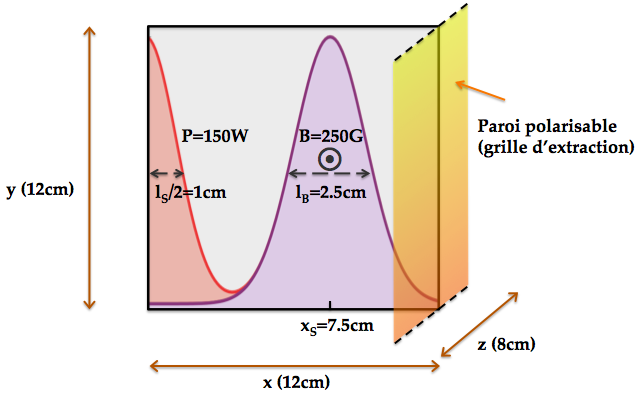
\includegraphics[width=0.7\textwidth]{figures/4-pegasesSimDomain.png}
{\caption{Le domaine de simulation est le plan perpendiculaire au champ
magnétique.}
\label{4-pegasesSimDomain}}
\end{figure}

Le domaine de simulation est rectangulaire et de
dimensions similaires à celles du prototype. La puissance est déposée dans la
région en amont du filtre magnétique sous la forme d'une demi-gaussienne de 2 cm
de largeur. Le filtre magnétique est aussi de forme gaussienne, centré en
$x_\mathcal{S}\,$= 7.5 cm et de largeur $l_\mathcal{S}\sim\,$2.5 cm. Les parois
seront choisies conductrices ou diélectriques, avec une polarisation éventuelle de la grille
d'extraction (en jaune à droite du domaine). La puissance totale absorbée et la
densité de gaz sont fixées respectivement à 250 W et 1 mTorr. Ces paramètre sont
résumés dans le tableau~\ref{4-PegasesParam1}.

\begin{table*}[!htbp]
\footnotesize\centering
\ra{1.3}
\begin{tabular}{cc}\toprule
\multicolumn{2}{c}{\bf Paramètres}\\
\midrule 
Parois & Isolantes\\
$L_x$, $L_y$ & 12cm\\
$L_z$ & 8cm\\
$B$&250G\\
$l_B$, $x_B$&2.5cm, 7.5cm\\
$\mathcal{P}_\text{ext}$&250W\\
$l_\mathcal{S}$, $x_\mathcal{S}$&2cm, 0cm\\
$\text{gaz (Ar)}$ & 1 mTorr\\
\bottomrule
\end{tabular}
\caption{Paramètres de la simulation.}\label{4-PegasesParam1}
\end{table*}

Les types de solutions obtenues par MAGNIS dans le cas de parois diélectriques
et sans bias appliqué sont illustrées figure \ref{2-CartesWithTe} :

\begin{figure}[!htbp]
    \centering
    \subfigure[]{\label{4-PegasesCarteDensiteBase}
    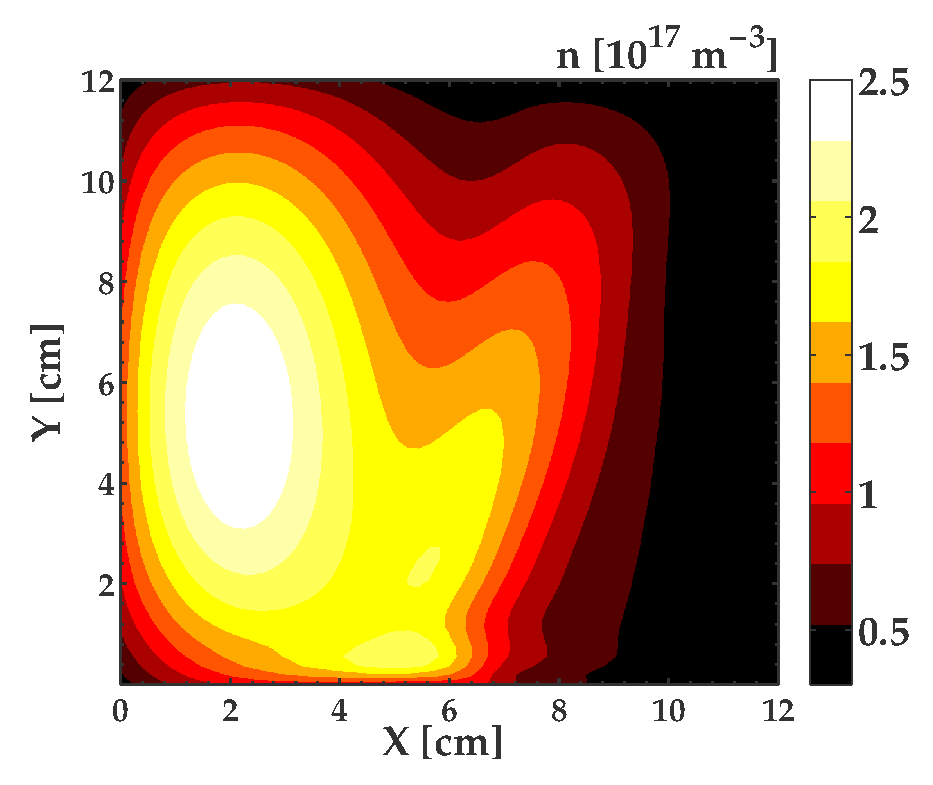
\includegraphics[height=5.75cm]{figures/4-PegasesCarteDensiteBase.eps}}
    \subfigure[]{\label{4-PegasesCartePotentielBase}
    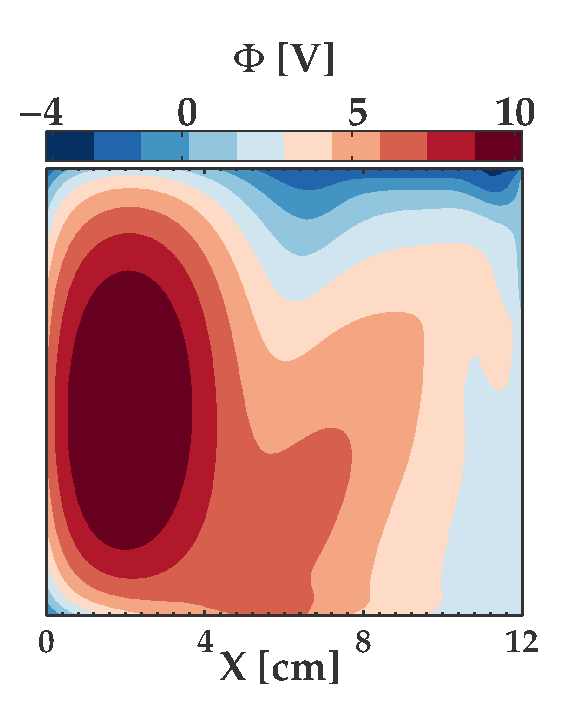
\includegraphics[height=5.75cm]{figures/4-PegasesCartePotentielBase.eps}}
    \subfigure[]{\label{4-PegasesCarteTemperatureBase}
    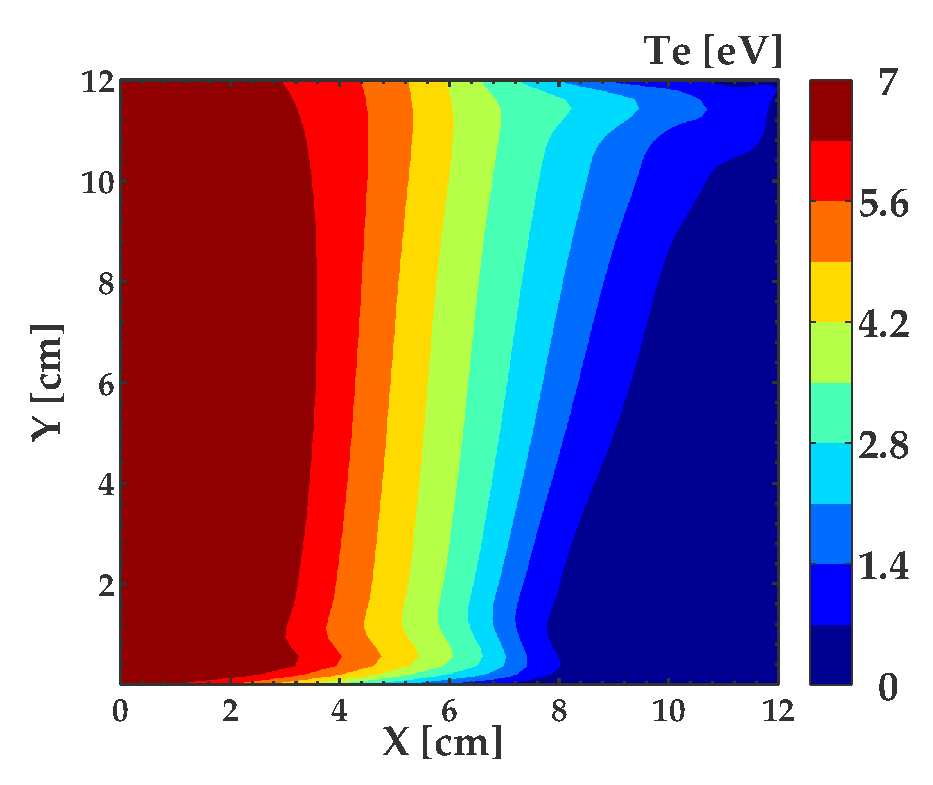
\includegraphics[height=5.75cm]{figures/4-PegasesCarteTemperatureBase.eps}}
    \caption{Cartes de densité \subref{4-PegasesCarteDensiteBase}~, de potentiel
    \subref{4-PegasesCartePotentielBase}~ et de température
    \subref{4-PegasesCarteTemperatureBase}~ dans le cas de parois
    diélectriques.}
    \label{2-CartesWithTe}
	\end{figure}

À partir de conditions initiales uniformes ($n_e\,$= 10$^{17}$ cm$^{-3}$ et
$T_e\,$= 5 eV), le plasma atteint un état stationnaire en $\tau\simeq\,$
10$^{-4}\,$s.
Le maximum de densité de la source, 2.5x10$^{17}\,$m$^{-3}$ est situé au
centre de la région d'ionisation. La densité du plasma décroît ensuite très
rapidement sur une longueur de 2 à 4 cm. 

\begin{figure}[!htbp]\centering
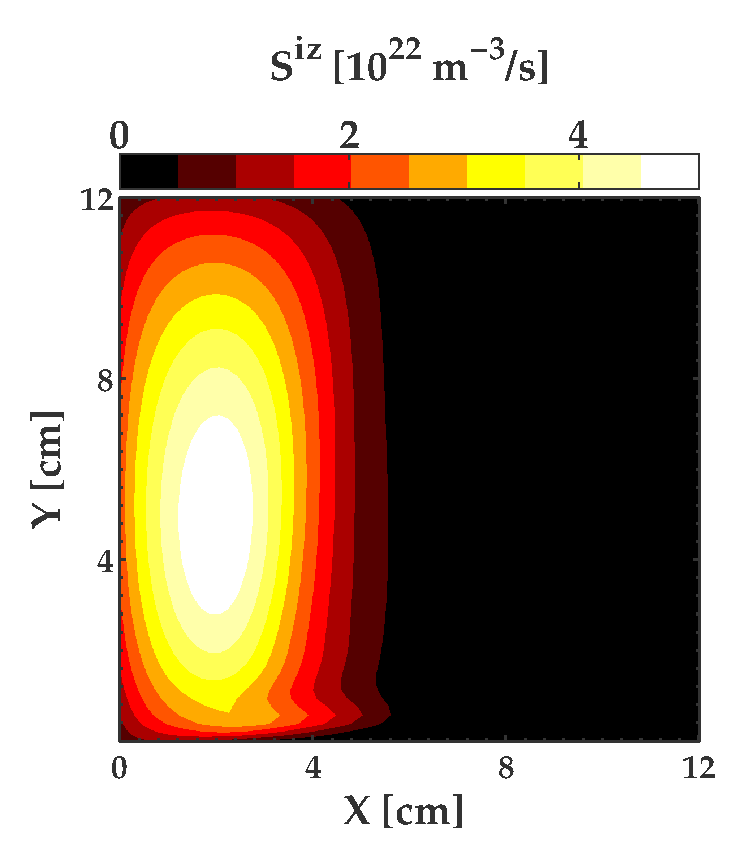
\includegraphics[height=6.5cm]{figures/4-PegasesCarteSourceBase.eps}
\caption{Source de particules provenant de l'ionisation.}
\label{4-PegasesCarteSourceBase}
\end{figure}

Sur la figure~\ref{4-PegasesCarteDensiteBase} on
observe aussi que le plasma s'étend jusque dans la région du filtre de façon
non-uniforme. L'origine de cette assymétrie sur la densité est liée
au transport du plasma : la figure~\ref{4-PegasesCarteSourceBase}, qui illustre
le nombre de particule ionisées par unité de temps et de volume, montre
que le plasma est créé en amont du champ magnétique, et que c'est donc principalement par un
processus de transport et non par un processus d'ionisation que le plasma arrive dans la région du
filtre.

La figure~\ref{4-PegasesCartePotentielBase} montre le potentiel
électrique $\Phi$. Il suit le profil de densité, et donne naissance à un champ
électrique d'une centaine de volt par mètre, quasiment ambipolaire dans la
région non magnétisée, et plutôt faible dans le filtre magnétique.

Enfin, une carte de la température électronique $T_e$ est présentée sur la
figure~\ref{4-PegasesCarteTemperatureBase}. De manière conforme à nos attentes,
le filtre magnétique fait fortement décroître la température électronique, la
faisant chuter de 7~eV à 1~eV sur une longueur de quelques centimètres : dans le
filtre, les électrons sont piégés le long des lignes de champ, ce qui
ralentit fortement leur déplacement et le transport
thermique dans la direction $x$.
On peut aussi remarquer une légère asymétrie qui se met en place le long de la
direction $y$.

Dans ce type de configuration
magnétique les électrons, dont la mobilité est considérablement réduite en
travers du champ magnétique, cherchent un moyen de franchir le filtre afin de
retrouver les ions et préserver la quasineutralité du plasma. Les cartes de flux
ioniques et électroniques présentées sur la figure~\ref{4-PegasesCarteFlux}
permettent de se faire une idée de la dynamique du système. 

\begin{figure}[!htbp]
  \centering
    \subfigure[]{\label{4-PegasesCarteFluxIBase}
    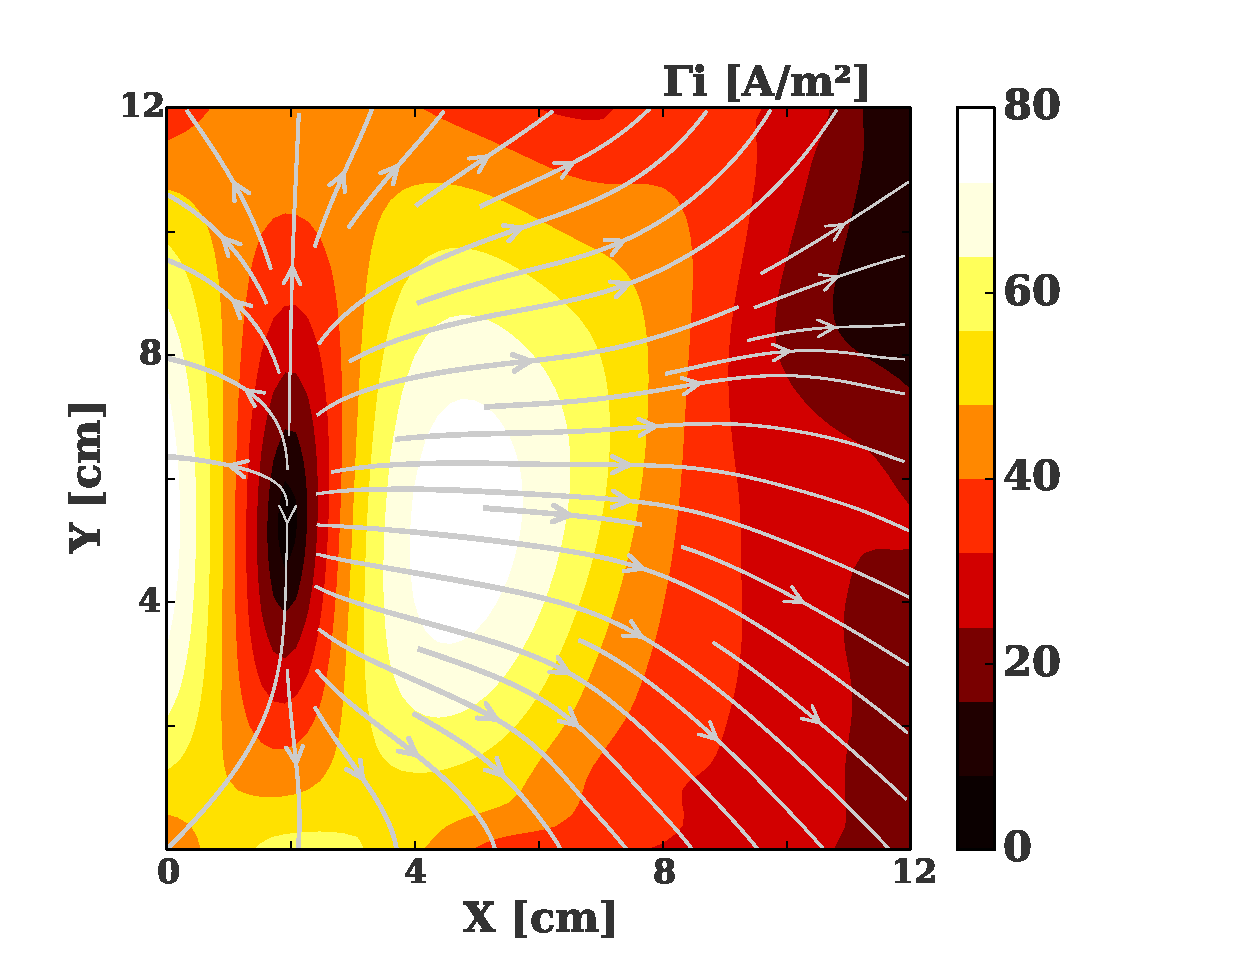
\includegraphics[height=6cm]{figures/4-PegasesCarteFluxIBase.eps}}
    \subfigure[]{\label{4-PegasesCarteFluxEBase}
    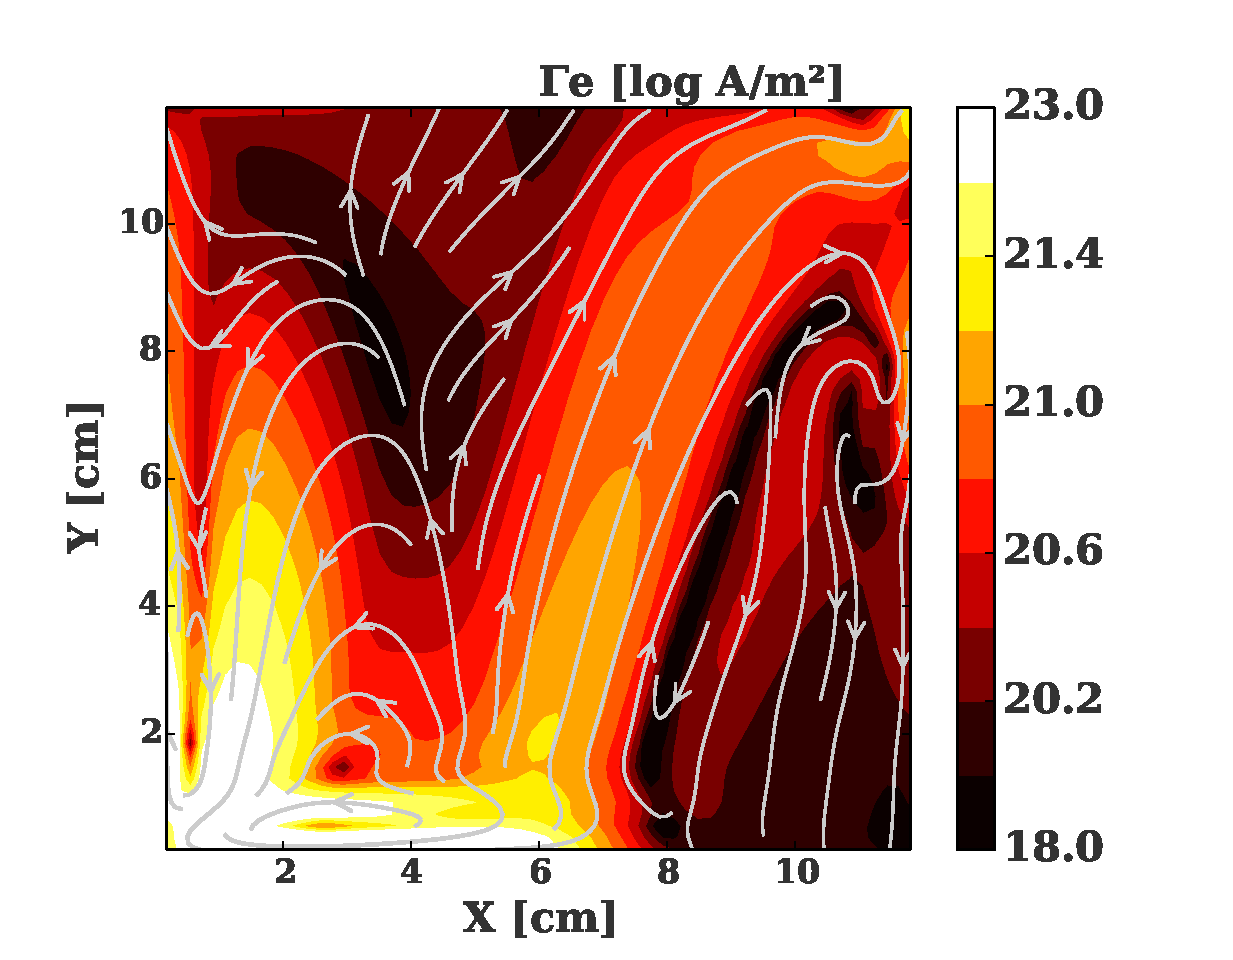
\includegraphics[height=6cm]{figures/4-PegasesCarteFluxEBase.eps}}
    \caption{Densité de courant ionique \subref{4-PegasesCarteFluxEBase}~
    et électronique \subref{4-PegasesCarteFluxEBase}~.}
    \label{4-PegasesCarteFlux}
\end{figure}

Dans la zone non
magnétisée, les ions issus de l'ionisation du gaz sont créés avec une vitesse
initiale quasiment nulle et tombent de façon rectiligne aux parois. Du côté
magnétisé, le flux augmente fortement puis diminue à travers le filtre (les
ions sont perdus le long des lignes), mais celui-ci n'a pas d'influence notoire sur la trajectoire des particules.

Le flux électronique est quant à lui bien moins évident à interpréter. La
caractéristique la plus immédiate à visualiser correspond au fort flux qui
remonte le long de la direction $y$. Ce comportement se retrouve dans d'autres
sources utilisant un filtre magnétique, notamment dans la
sources d'ions négatifs de Garching~\parencite{Fantz} et a été modélisé
dans ce contexte à travers différents
modèles, fluides et cinétiques~\parencite{PIC2D,PIC3D,MAGMA}. 

On peut remarquer
deux autres phénomènes, moins détaillés dans la littérature : tout d'abord il
faut noter que le flux le plus important se situe dans la zone non magnétisée au
niveau de la paroi dans la région que nous appelerons basse de la source (en
$y\sim\,$0~cm).
La figure~\ref{4-PegasesCarteFluxEBase} montre que le flux électronique
traversant le filtre prend sa source dans la région basse du filtre, qui
s'alimente à son tour en attirant le plasma le long de la paroi.
Le deuxième point concerne la région en aval du filtre, où l'on observe que le
flux électronique traverse le domaine en sens inverse, une partie de celui-ci franchissant même à nouveau
la barrière magnétique au niveau de la paroi opposée.

\subsection{Étude paramétrique}
Dans cette partie, nous
réalisons une étude paramétrique sur les paramètres suceptibles
d'influencer le comportement du plasma dans le propulseur. Nous faisons varier
la pression de gaz, le profil de dépôt de puissance ainsi que la forme et
l'intensité du champ magnétique dans un plasma d'argon pur. Les paramètres et
les plages de valeurs qui ont été regardés correspondent à ceux testés par Jérôme Bredin pendant une étude sur la
chute de température électronique en présence d'un champ magnétique
non-uniforme~\parencite{Bredin}, nous donnant ainsi une base intéressante pour
tester et discuter les résultats du modèle.

Dans ces expériences, la grille d'extraction est
enlevée, la source étant reliée à un grand volume diminuant l'expansion spatiale du plasma. Pour nous
placer au plus près des conditions expérimentales, le domaine est allongé dans
la direction $x$ jusqu'à une longueur de 18~cm. Les parois sont quant à elle
choisies diélectriques. Les profils sont pris dans la direction $x$, au niveau
du milieu de la source (en $y\,=$ 6~cm) et il faut donc garder en tête la
présence de l'assymétrie générale du plasma, qui n'apparaît pas sur ces coupes.
	
\subsubsection{Scan en pression}

Nous regardons tout d'abord l'effet de la pression du gaz, choisie
successivement à 1 mTorr, 10 mTorr et 100 mTorr, sur le transport du plasma.
Les paramètres des simulations sont rappelés dans le
	tableau~\ref{4-PegasesScanPreParam}.
	
	 La
	figure~\ref{4-pegasesCompPressDenProfile} montre une comparaison des profils de densité. Ces profils sont plutôt en bon accords avec les
	mesures :
	à 100~mTorr, la densité du plasma atteint 10$^{18}$~m$^{-3}$ puis décroît
	exponentiellement.  La température électronique reste approximativement égale à
	2~eV et n'est que faiblement impactée par le filtre magnétique.
	\bigskip
	
\begin{minipage}{\textwidth}
\footnotesize\centering
\ra{1.3}
\begin{tabular}{lcclc}\toprule
\multicolumn{5}{c}{\bf Paramètres}\\
\midrule 
Parois & Isolantes &&$L_x$, $L_y$, $L_z$  & 12cm, 12cm,
8cm\\
$\mathcal{P}_\text{ext}$&250W&&$l_\mathcal{S}$, $x_\mathcal{S}$&2cm, 0cm\\
$B$&250G&&$l_B$, $x_B$&2.5cm, 7.5cm\\

\textbf{gaz (Ar)} & \textbf{1--100 mTorr}&&&\\
\bottomrule
\end{tabular}
\captionof{table}{Paramètres de la simulation.}\label{4-PegasesScanPreParam}
\end{minipage}
	
\begin{figure}[!htbp]
  \centering
    \subfigure[]{\label{4-pegasesCompPressDenProfile}
    
\includegraphics[height=5cm]{figures/4-pegasesCompPressDenProfile.eps}}
    \subfigure[]{\label{4-pegasesCompPressTempProfile}
    
\includegraphics[height=5cm]{figures/4-pegasesCompPressTempProfile.eps}}
    \caption{Profils de densité~\subref{4-pegasesCompPressDenProfile}~ et de
    température~\subref{4-pegasesCompPressTempProfile}~ pour trois pressions de
    gaz différentes, 1 mTorr, 10 mTorr et 100 mTorr.}
    \label{pegasesCompPressProfils}
\end{figure}
	
	La figure~\ref{4-pegasesCompPressTempProfile} montre le profil de température. Bien
	plus élevée à basse pression, $T_e$ part d'un maximum de 7~eV à $x\,$= 2~cm et
	diminue à travers le filtre pour atteindre une valeur constante d'environ 1~eV
. On note cependant que le minimum de température n'est pas atteint exactement
au même niveau que dans les expériences, celles-ci le plaçant au centre de la
barrière magnétique, et le modèle le prédisant plutôt à la fin du filtre (cette
différence pouvant éventuellement être imputée à la géométrie du champ
magnétique, rectiligne dans le modèle).

	\subsubsection{Variations du champ magnétique}
	
	La comparaison des profils à différents champs magnétiques, présentée
	figure~\ref{4-pegasesCompMagProfile}, est un peu moins concordante. Les mesures
	expérimentales montrent en effet une augmentation de la densité et une
	température post-filtre de 2 eV. Cependant, lors des mesures à 140 G
	d'intensité de champ, on voit que le profil du filtre est aussi un peu plus
	large, pouvant éventuellement influencer les paramètres du plasma.
	
\begin{figure}[!htbp]
  \centering
    \subfigure[]{\label{4-pegasesCompMagDenProfile}
    
\includegraphics[height=5cm]{figures/4-pegasesCompMagDenProfile.eps}}
    \subfigure[]{\label{4-pegasesCompMagTempProfile}
    
\includegraphics[height=5cm]{figures/4-pegasesCompMagTempProfile.eps}}
    \caption{Profils de densité \subref{4-pegasesCompMagTempProfile}~ et de
    température \subref{4-pegasesCompMagTempProfile}~ pour trois intensité de
    champ magnétique 50G, 140G et 250G.}
    \label{4-pegasesCompMagProfile}
\end{figure}

Pour confirmer ces hypothèses, faisons varier $l_\mathcal{S}$ la largeur de
dépôt d'énergie et $l_B$ la largeur de la barrière pour deux
intensités de champ magnétique puis comparons la densité maximale et la température des électrons après le
filtre. On voit dans le tableau \ref{4-pegasesCompLargeurs} que quand le
filtre est plus long, la densité augmente et la température baisse de façon plus
prononcée.
De l'autre côté, quand l'énergie est déposée sur une plus grande distance, la
densité a plutôt tendance à diminuer tandis qu'après la barrière, la
température électronique remonte.

\begin{table}
\footnotesize\centering
\ra{1.3}
\begin{tabular}{@{}ccccccc@{}}\toprule
\bfseries B&&\multicolumn{2}{c}{$l_B=2cm$} && \multicolumn{2}{c}{$l_B=4cm$}\\
\cmidrule{3-4} \cmidrule{6-7}
&& $n (m^{-3})$ & $\min T_e (eV)$ && $n (m^{-3})$ & $\min T_e (eV)$\\
\midrule 
250G\\
\scriptsize $l_\mathcal{S}=2cm$ &&\bfseries\scriptsize 1.58
10\textsuperscript{17}&\bfseries\scriptsize 0.91&&\scriptsize 2.3
10\textsuperscript{17}&\scriptsize 0.73
\\
\scriptsize $l_\mathcal{S}=4cm$  &&\scriptsize 1.4 10\textsuperscript{17}
&\scriptsize 2.08&&\scriptsize 12 10\textsuperscript{17}&\scriptsize 1.38\\
140G\\
\scriptsize $l_\mathcal{S}=cm$ &&\scriptsize 1.57 10\textsuperscript{17}
&\scriptsize 1.27&&\scriptsize 1.96 10\textsuperscript{17}&\scriptsize 0.98 \\
\scriptsize $l_\mathcal{S}=4cm$  &&\scriptsize 1.39 10\textsuperscript{17}
&\scriptsize 2.36&&\bfseries\scriptsize 1.75 10\textsuperscript{17}&\bfseries\scriptsize
1.6\\
\bottomrule
\end{tabular}
\caption{Tableau comparatif présentant la densité maximale du plasma ainsi que
la température électronique après le filtre magnétique pour des largeurs de
source d'énergie $l_S$ et de filtre magnétique $l_B$ différentes.}
\label{4-pegasesCompLargeurs}
\end{table}

Dans les mesures réalisées sur PEGASES, le filtre magnétique est respectivement
de largeur 4 cm et 2 cm dans les cas à 140 G et 250 G, ne laissant que deux
résultats "possibles" à prendre en considération. 
Les valeurs se rapprochant le plus des données expérimentales sont en gras dans
le tableau, elles correspondent à une largeur de source plus petite dans le cas fortement
magnétisé et inversement à une largeur de puissance déposée plus grande quand le
champ magnétique est plus étendu. L'influence de la taille de la zone de
chauffage n'est donc pas négligeable dans le cas des sources d'ion et semble de
plus varier en fonction de la configuration magnétique.

\subsection{Transport du courant dans le cas de parois conductrices et d'un bias
appliqué}

La suite de cette étude porte sur le cas de parois
conductrices. Dans cette configuration, représentative de
l'un des modes de fonctionnement de PEGASES ainsi que de nombreuses
expérimentations, l'application d'un bias positif sur la grille d'extraction afin d'extraire un
courant d'ions négatifs modifie aussi de manière conséquente les boucles de
courant dans le plasma (dans la source de Garching, on joue sur le bias pour
optimiser les flux). Le transport du courant est régit par l'équation de
conservation du courant :

\begin{equation}
\nabla\cdot\mathbf j=\nabla_\para\cdot \mathbf j_\para +\nabla_\perp\cdot
\mathbf j_\perp
\end{equation}

L'image simple d'un transport du courant homogène et
ambipolaire (et éventuellement fortement réduit par un champ magnétique dans la
direction perpendiculaire) est totalement trompeuse. Il est clair aujourd'hui
que ce transport de courant, même en l'absence de champ magnétique, est bien plus difficile à appréhender, le
courant formant des boucles et des vortex (tourbillons) et pouvant
éventuellement se refermer dans des parois conductrices (effet Simon~\parencite{Simon55}).

Cet effet est particulièrement déterminant pour le transport global du
plasma en présence d'un champ magnétique ; les électrons, qui auront plutôt
tendance à faire passer le courant par les parois qui
interceptent les lignes de champ magnétique, court-circuitent l'intérieur du
plasma. La gaine au bout des lignes de champ joue alors un rôle crucial dans
l'évolution du potentiel, et ce jusqu'au c\oe{}ur de la source. A basse
pression, les solutions deviennent instationnaires, et le transport change
radicalement de nature, devenant instable avec des phénomènes instationnaires
et réguliers.
	
\subsubsection{Influence du champ magnétique}
Dans les sources d'ions utilisant un filtre magnétique, on soupsonne le flux
d'électrons d'être le principal responsable de l'inhomogénéité
de densité observée~\parencite{PIC2D,PIC3D}.
Notons le courant total d'électron récupéré à la paroi par :

\begin{equation}
I=\int\int J_e\text{dA}
\end{equation}
\begin{minipage}{\textwidth}
\footnotesize\centering
\ra{1.3}
\begin{tabular}{lcclc}\toprule
\multicolumn{5}{c}{\bf Paramètres}\\
\midrule 
Parois & Conductrices &&$L_x$, $L_y$, $L_z$  & 12cm, 12cm,
8cm\\
$\mathcal{P}_\text{ext}$&250W&&$l_\mathcal{S}$, $x_\mathcal{S}$&2cm, 0cm\\
$B$&\textbf{0--250 G}&&$l_B$, $x_B$&2.5cm, 7.5cm\\
$\Phi_w$ & \textbf{0--20 V}&&gaz (Ar) & 1 mTorr\\
\bottomrule
\end{tabular}
\captionof{table}{Paramètres de la simulation.}\label{4-PegasesScanPreParam}
\end{minipage}

$I$ est théoriquement réduit d'un facteur en $1/B^2$ à travers le filtre dans
une analyse unidimensionnelle (ne tenant pas compte de la direction de dérive
$y$). On peut voir sur la figure~\ref{pegasesVarMagCourantParoi} le courant
total $I$ récupéré au niveau de la grille d'extraction (sur le bord droit du
domaine) : sans bias appliqué, $I$ suit à peu près cette loi d'échelle en
$1/B^2$. Cependant, quand le bias augmente, on voit que le $I$ commence plutôt à suivre une loi en
$1/B$. Cette variation en $1/B$ est généralement prise comme la signature de la
présence d'un transport anormal.

Pourtant, dans ces sources, le transport reste classique et la raison de cette
augmentation significative doit être recherchée dans les effets induits par les
dérives  magnétiques. Nous ne nous tenterons pas à
expliquer l'origine de ce transport (bien que la future utilisation de MAGNIS
sera possiblement d'une grande utilité pour aider à répondre à cette question).
Actuellement, même si les tentatives d'explications s'accordent sur la
traversée du filtre des électrons via la forte dérive ExB à proximité de la
gaine, la déviation d'origine du flux électronique en face du filtre reste à
l'origine de nombreux débats.

\begin{figure}[!htbp]
	\centering
	
\includegraphics[width=0.6\textwidth]{figures/4-pegasesVarMagCourantParoi.eps}
	{\caption{Courant total d'électrons récupéré à la paroi $I$ en fonction de l'intensité du filtre magnétique pour trois
	voltages appliqués (0 V, 10 V et 20 V). }
	\label{pegasesVarMagCourantParoi}}
	\end{figure}

Attardons nous donc sur le flux électronique, à travers l'augmentation
progressive de l'intensité du champ magnétique. La
figure~\ref{4-pegasesfluxElectronique} représente une comparaison croisée du
flux d'électrons pour un champ magnétique variant de 0 G à 500 G et trois bias
différents de 0 V, 10 V et 20 V appliqués à la grille d'extraction de la source. 

Les trois premières cartes, en l'absence de filtre magnétique, montrent la
situation initiale pour les trois différents voltages. Basiquement, on observe
que l'application du bias attire le flux électronique qui peut alors atteindre
dans le plasma une densité de courant de l'ordre de $\sim$10$^2$ A/m$^2$ et que
le flux à la paroi est uniforme\footnote{Cette
situation, bien que basique, est déjà intriguante en soi : le flux électronique
forme des vortex en dehors de la région d'ionisation et remonte le long des
gradient de densité. Ce phénomène est hors de contexte du présent
manuscrit mais mérite tout de même d'être signalé, étant totalement absent de
la littérature.
Des simulations PIC ont par ailleurs montré un comportement
similaire~\parencite{PIC3D}.}.

 \begin{figure}[!htbp]
	\centering
	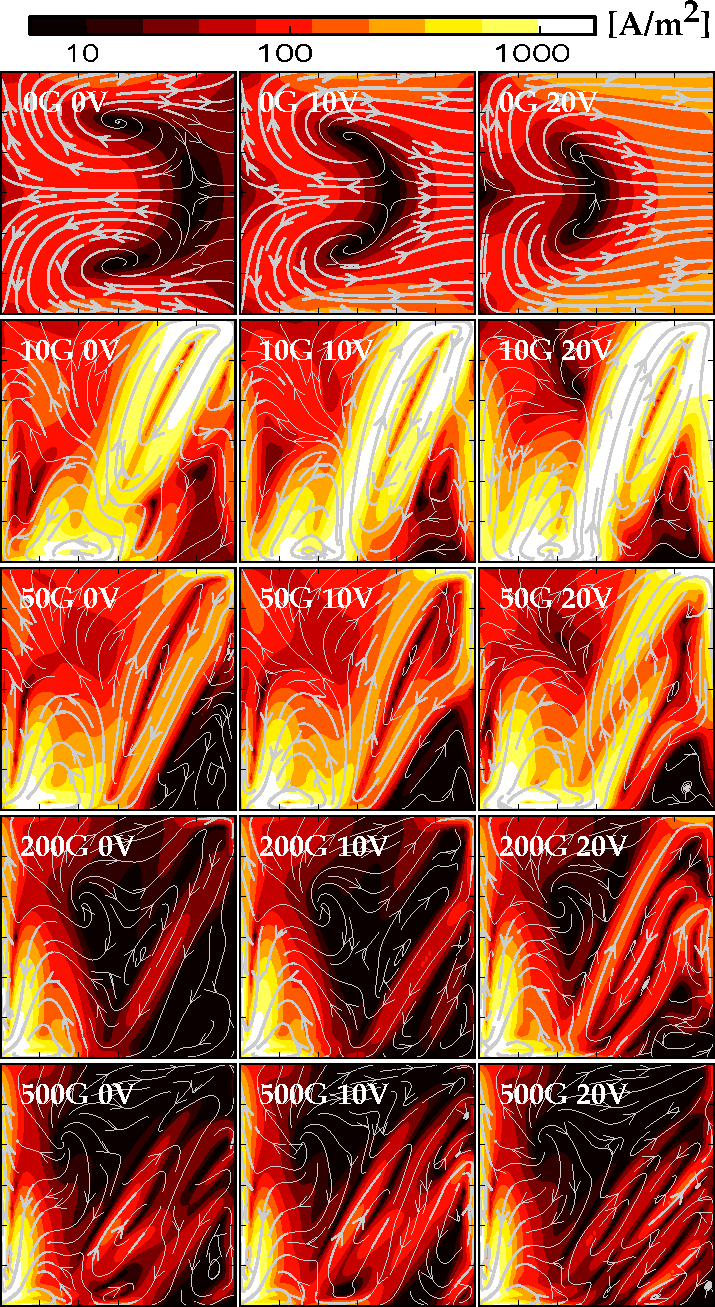
\includegraphics[width=0.85\textwidth]{figures/4-pegasesfluxElectronique.pdf}
	{\caption{Flux électronique à travers le filtre magnétique sur une plage
	allant de 0 G à 500 G pour trois voltages appliqués sur la grille
	d'extraction (sur le bord droit du domaine) différents 0 V, 10 V et 20 V.}
	\label{4-pegasesfluxElectronique}}
	\end{figure}
	
L'application d'un filtre magnétique, même à faible intensité de champ, modifie
complètement le flux électronique : la densité de courant devient asymétrique et
décuple d'intensité dans le bas de la région d'ionisation. À 10 G, la
température électronique est de l'ordre de 5 eV, donnant un rayon de Larmor
électronique d'environ 5 mm. Les électrons sont déjà magnétisés et ne peuvent
traverser le filtre qu'au niveau de la paroi située en $y\,$=12 cm. Le flux
d'électrons se sépare ensuite pour rejoindre les ions qui ont traversé la
barrière sans perturbation, une partie plus ou moins importante allant à la
paroi en fonction du bias et l'autre traversant le domaine en sens inverse
jusqu'à atteindre la paroi en $y\,$= 0 cm.

À 50 G, l'intensité du courant électronique reste importante et un phénomène de
circulation des électrons autour de la barrière magnétique devient plus clair.
L'application du bias montre aussi que le flux est dévié et longe la grille
d'extraction sur quelques centimètres en direction de la partie basse du filtre.
À 200 G et sans bias appliqué, le flux électronique est fortement réduit à travers la barrière et change encore de
forme : le premier courant qui remontait le long du champ magnétique devient
moins important que le flux de retour en bas de la barrière. L'application d'un
bias ou l'augmentation de l'intensité du champ magnétique mène alors à
l'apparition d'un phénomène instable que nous allons regarder plus en détail dans la partie suivante.

Plus généralement, sur l'ensemble des cas présentés avec $B\neq\,$0, on remarque
que le bias ne change pas radicalement les profils du flux.

\subsection{Phénomènes intermittents, instabilités}
À faible champ magnétique ou à pression suffisamment élevée, les solutions
obtenues par MAGNIS sont stationnaires.
Cependant, lorsque la pression diminue, le transport collisionnel n'est plus
dominant et des phénomènes instables, caractéristiques des plasmas
magnétisés, peuvent apparaître et affecter toute la dynamique du système. 
 
\subsubsection{Vagues ioniques}
La première instabilité que l'on voit apparaître est illustrée
figure~\ref{4-PegasesCarteDensiteWaves}. À intervalles régulières, des bouffées
de plasma traversent le filtre magnétique à des vitesses de l'ordre de la
vitesse de Bohm du système.
La direction de propagation est perpendiculaire au front de densité, à l'oblique entre le champ magnétique et son gradient. Sans bias et à une pression de gaz de 1mTorr,
 les fronts de densité apparaissent à une fréquence d'environ 120kHz et se
 déplacent à une vitesse approximative de 2.10$^3$ m.s$\puissance{-1}$. 
 
\begin{figure}[!htbp] 
  \centering
    \subfigure[]{\label{4-PegasesCarteDensiteWaves}
    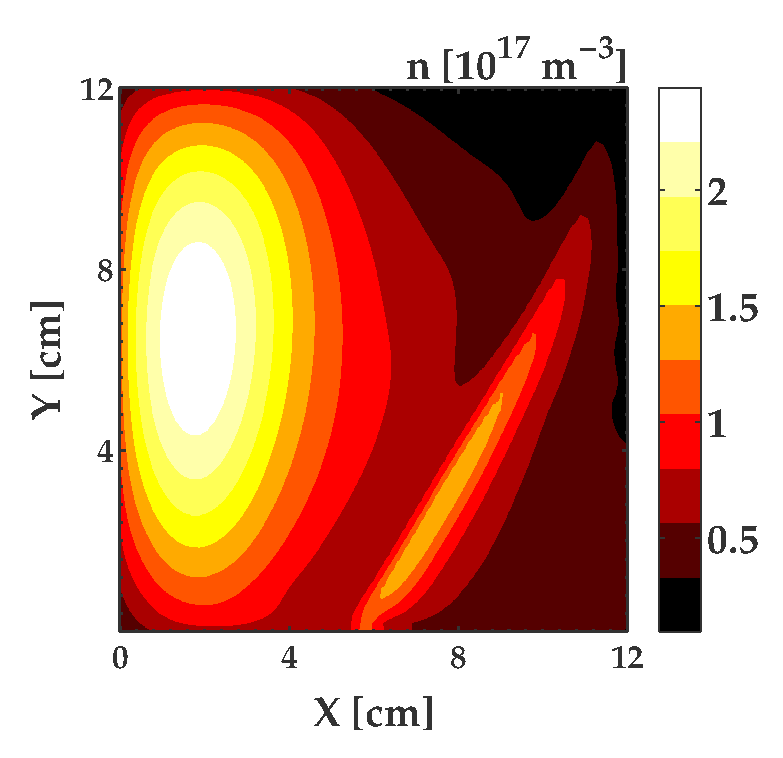
\includegraphics[height=5cm]{figures/4-PegasesCarteDensiteWave.eps}}
    \subfigure[]{\label{4-PegasesCarteViSurTeVarBias}
    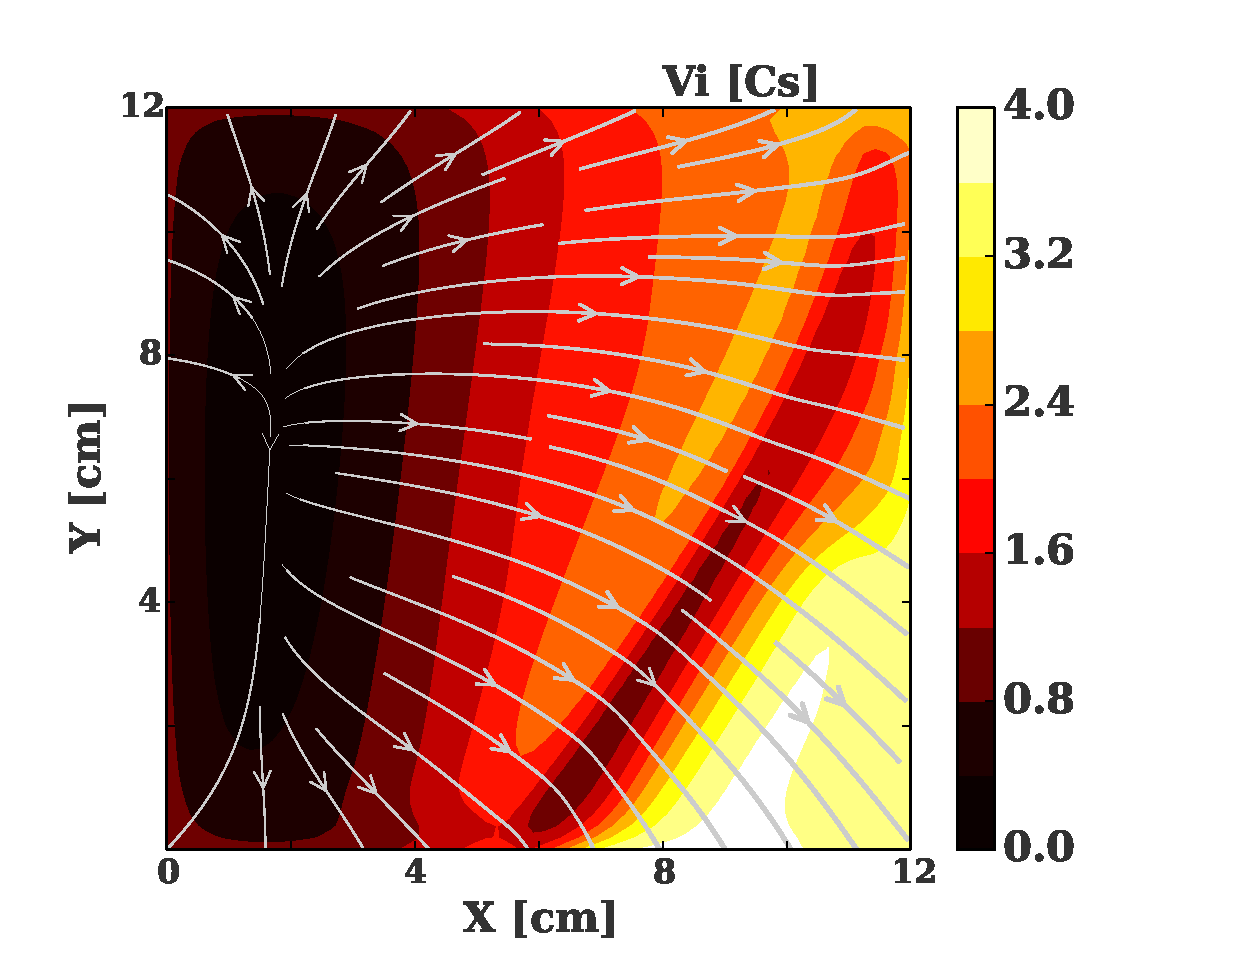
\includegraphics[height=5cm]{figures/4-PegasesCarteViSurTeVarBias.eps}}
    \caption{Cartes de la densité plasma~\subref{4-PegasesCarteDensiteWaves}~ et
    de vitesse ionique rapportée à la
    vitesse de Bohm locale
    $c_s=\sqrt{T_e/m_i}$~\subref{4-PegasesCarteViSurTeVarBias}~ pour un champ
    magnétique de 250 G, une densité d'argon de 1mTorr et un bias appliqué de
    20V.}
    \label{4-PegasesVaguesIoniques}
\end{figure}
 
 La figure~\ref{4-PegasesCarteViSurTeVarBias} représente la vitesse ionique
 rapportée à la vitesse de Bohm, ie. le nombre de Mach de
 l'écoulement ionique. On voit tout d'abord qu'une grande partie du domaine est
 occupée par des ions dont la vitesse dépasse la vitesse de Bohm locale. En
 effet, les ions franchissent le seuil $v_i=c_s$ (Mach1) le long du gradient de
 température, à $T_e\sim\,$5 eV puis accélèrent encore jusqu'à atteindre
 $v_i=2c_s$ (Mach2) avant le front de densité. La vitesse décroît ensuite lors
 de la traversée de la bouffée, tout en restant de l'ordre de la vitesse de
 Bohm.
 
 La vitesse de phase $v_\phi$ calculée ($v_\phi\sim\,$2.10$^3$
 m.s$\puissance{-1}$) , représentative de la propagation de la bouffée, est inférieure à la
 vitesse des particules la constituant ($u_i\sim\,$4.10$^3$
 m.s$\puissance{-1}$). Très naïvement, ce phénomène fait penser aux phénomènes
 de compression-décompression liés aux ondes soniques dans les gaz
 classiques, où le front de densité serait l'onde acoustique
 résultante du passage des ions supersoniques. En supposant que la vitesse de
 propagation de l'onde est caractéristique de cette transition (dans
 l'analogie, les ondes sonores se déplacent à la vitesse du son), il est tentant de définir la température correspondante à $v\phi$ :
 
 \begin{equation}
 	v_\phi=c_{s}=\sqrt{\frac{T_e}{m_i}}\simeq 2.2\;10^{3}\,\text{m.s}^{-1}
 	\Leftrightarrow T_e\simeq 2\,\text{eV}
 \end{equation}
 
 Quelques propriétés peuvent être immédiatement dégagées. L'apparition de cette
 instabilité et certaines de ses particularités sont directement reliées au
 gradient de température électronique et au terme d'inertie :
 
 \begin{itemize}
   	\item Les solutions du modèle quand le terme inertiel d'advection est
	négligé sont stationnaires.
   \item Un plasma isotherme s'étend dans le filtre dans la direction du flux
   d'électrons transverse et atteint lui aussi une solution stationnaire.
   \item la direction des fronts d'ondes est fortement corrélée au gradient
   de température.
\end{itemize}

La réponse à la polarisation de la grille d'extraction est aussi une
caractéristique intéressante de ce phénomène. Les
figures~\ref{4-PegasesCarteDensiteVarBiasWave}~
\subref{4-PegasesCarteDensiteVarBias1}~ \subref{4-PegasesCarteDensiteVarBias2}~
et~\subref{4-PegasesCarteDensiteVarBias3}~ illustrent cet effet en partie : la
dynamique des fronts, de vitesse de phase $v_\phi$ approximativement constante à
0 V, se décompose en deux temps après l'application d'un faible voltage. Les
fronts ralentissent au niveau du maximum du filtre magnétique, augmentent en densité, puis sont
propulsés vers les parois après un certain temps de latence. À 30 V, en
l'absence de champ accélérateur, un bras de plasma se forme en travers du
filtre, de densité équivalente à celle du plasma de la région d'ionisation.
	
	\begin{figure}[!htbp]
  \centering
    \subfigure[]{\label{4-PegasesCarteDensiteVarBias1}
    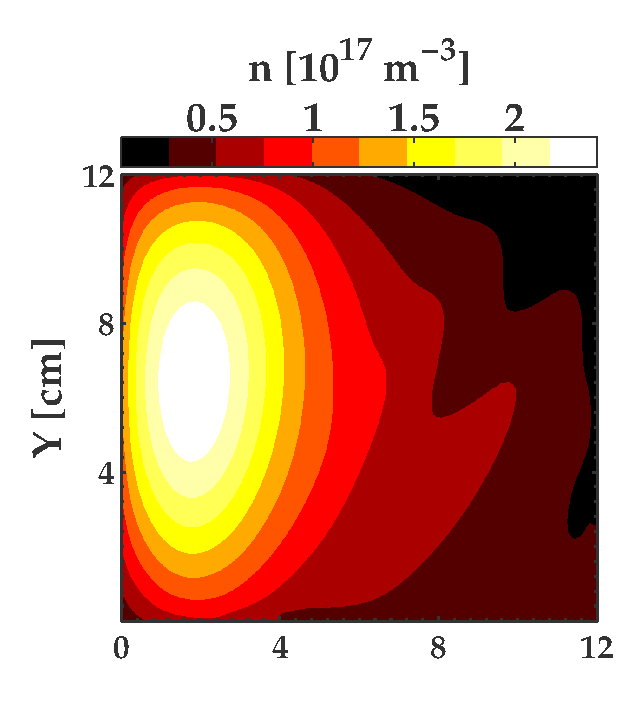
\includegraphics[height=6cm]{figures/4-PegasesCarteDensiteVarBias1.eps}}
    \subfigure[]{\label{4-PegasesCarteDensiteVarBias2}
    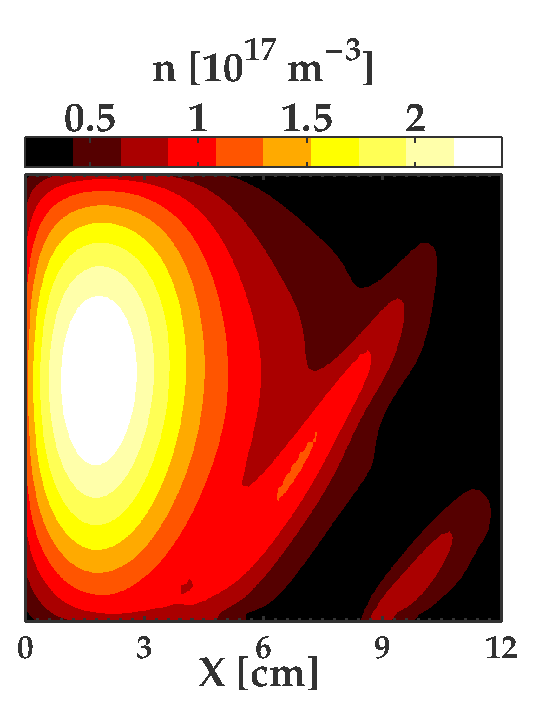
\includegraphics[height=6cm]{figures/4-PegasesCarteDensiteVarBias2.eps}}
    \subfigure[]{\label{4-PegasesCarteDensiteVarBias3}
    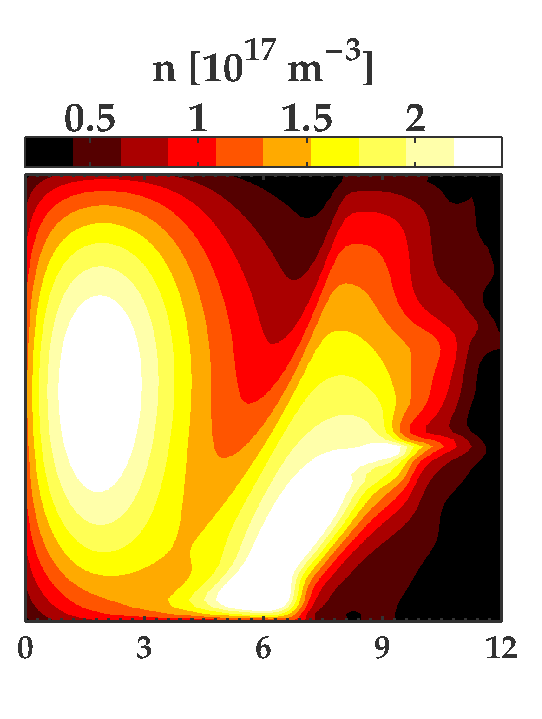
\includegraphics[height=6cm]{figures/4-PegasesCarteDensiteVarBias3.eps}}
    \caption{Cartes de densité\subref{4-PegasesCarteDensiteVarBias1}~, de
    potentiel\subref{4-PegasesCarteDensiteVarBias2}~ et de
    température\subref{4-PegasesCarteDensiteVarBias3}}
    \label{4-PegasesCarteDensiteVarBiasWave}
\end{figure}

On peut maintenant préciser la forme du flux électronique 
dans les cas fortement magnétisés de la
figure~\ref{4-pegasesfluxElectronique}. Un champ électrique apparaît
entre les fronts de densité, et se combine au filtre
magnétique pour faire naître un mouvement de dérive du type ExB, amplifiant le
transport des électrons au travers de la barrière. 

Enfin, il faut toutefois relever que le modèle n'arrive pas à trouver 
de fréquence ou de longueur d'onde caractéristique pour ces oscillations,
celles-ci variant en fonction de la taille du maillage. La
vitesse des particules ainsi que celle des fronts d'onde semblent quant-à
elles indépendantes du maillage.
La caractérisation complète de cette instabilité est donc pour le moment
assez difficile à réaliser.

Pour terminer, on peut se poser la question de la réalité physique de
ce phénomène, qui n'a apparemment pas été remarqué lors des expérimentations. La
présence d'ions supersoniques ne serait pourtant pas surprenante, étant donné
les gradients extrêmes, la très faible température électronique 
après le filtre, et la forte tension retenant le flux ionique.
Des simulations PIC, récemment lancées au GREPHE sur une géométrie similaire
à notre configuration, semblent montrer un comportement similaire, ce qui nous
conforte dans les résultats du modèle.

	\subsubsection{Peigne de densité}
	A plus haute pression (10 mTorr et 100 mTorr), l'application d'un bias positif
	à la grille d'extraction révèle une autre instabilité qui prend la forme d'un
	"peigne" (cf.
	figure~\ref{4-PegasesCarteDensiteVarBias5}). On peut aussi la voir apparaître :
	
	\begin{itemize}
	  \item le long des fronts de densité
	  \item au niveau des parois
	  \item dans des simulations isothermes
	  \item dans un champ magnétique uniforme (cas de la colonne de plasma)
	\end{itemize}
		
\begin{figure}[!htbp]
  \centering
    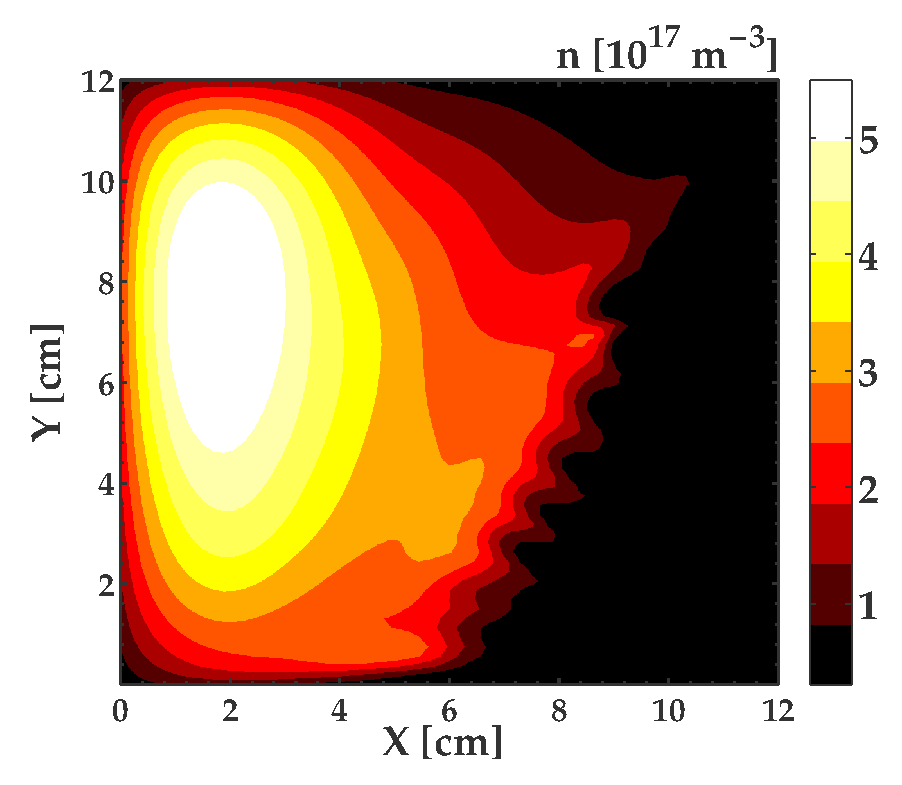
\includegraphics[height=5cm]{figures/4-PegasesCarteDensiteVarBias5.eps}
    \caption{Carte de densité pour une pression de gaz de 10 mTorr et un bias
    de 30 V appliqué à la grille
    d'extraction.\label{4-PegasesCarteDensiteVarBias5}}
\end{figure}
	
	Ce phénomène, qui se développe sur les bords du plasma et
	en présence d'un champ électrique important, rappelle
	les travaux de Simon~\parencite{Simon63} dans lesquels il démontre que l'état
	stationnaire peut devenir instable si le signe du produit du
	gradient de densité et du champ électrique est positif :
	
	\begin{equation}
		\nabla n\cdot \mathbf E>0
	\end{equation}
	
	Le champ électrique requis est dans la direction opposée à celle du champ
	électrique ambipolaire confinant usuellement les plasmas froids. Si l'étude de
	Simon nous renseigne sur l'un des ingrédients de cette instabilité, elle porte
	cependant sur un plasma isotherme et dans une géométrie simplifiée par rapport
	à notre cadre d'étude. L'étude linéaire se complexifie hélas fortement avec la
	prise en compte de la température électronique et la présence d'un gradient
	de champ magnétique, rendant l'étude analytique de ce phénomène problématique.

	Dans cette partie, nous avons tout d'abord donné des éléments pour
	valider le modèle dans une configuration de filtre magnétique. Nous avons ainsi
	montré que MAGNIS pouvait reproduire le comportement du flux électronique et
	l'inhomogénéité du plasma dans le plan perpendiculaire au champ
	magnétique. Nous avons aussi donné les premiers constats de la présence d'ions
	supersoniques et d'un transport instationnaire à travers le filtre.
	Malgré les problèmes de convergence qui nous font douter de la nature physique
	ou numérique des instabilités, il est très difficile les faire
	totalement disparaître en jouant sur les paramètres.
	
\section{Colonne de plasma magnétisée - Cybele}

Cybele, présentée sur la figure~\ref{4-cybelePhoto}, est une source d'ions
négatifs de dimension très allongée développée à
l'IRFM (CEA)~\cite{Simonin} dans le cadre de la recherche sur les systèmes
d'injection de neutres (IDN) qui sont utilisés pour le chauffage et la
génération de courant dans les réacteurs de fusion par confinement magnétique\footnote{Le principe d'un
injecteur de neutres est basé sur l'accélération d'ions à très haute énergie,
puis neutralisés afin de former un puissant faisceau de neutres.
Le faisceau est ensuite injecté au c\oe{}ur du réacteur pour déposer son énergie
directement dans le plasma. Pour ITER, les deux IDN devront fournir 17MW de
puissance chacun, en injectant 40A de D$\puissance{0}$ à
1MeV~\parencite{Hemsworth}.}.

\begin{figure}[!htbp]
  \centering
  \subfigure[]{\label{4-cybelePhoto}
    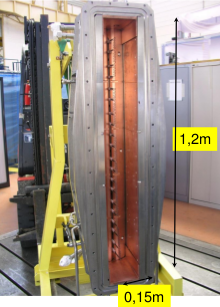
\includegraphics[height=8cm]{figures/4-cybelePhoto.png}}
    \subfigure[]{\label{4-CybelePhoto2}
    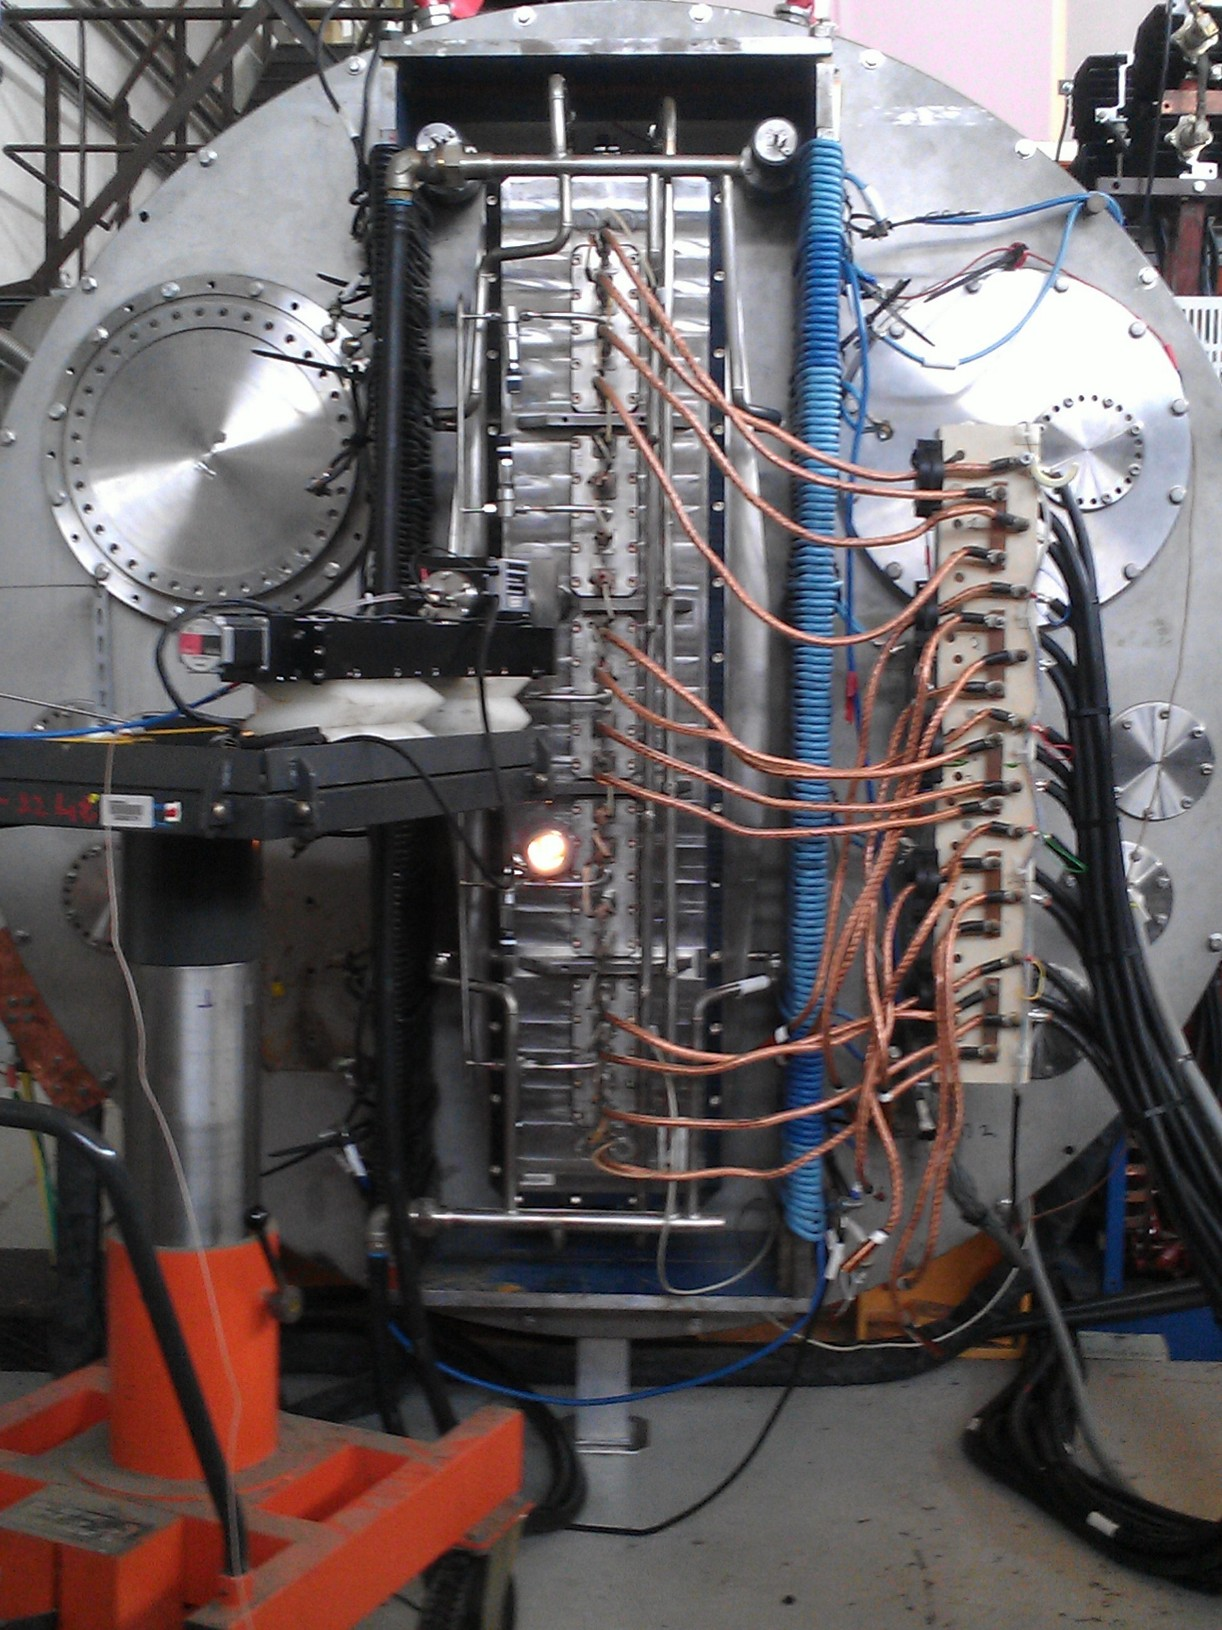
\includegraphics[height=8cm]{figures/4-CybelePhoto2.jpg}} 
    \caption{Photographies de la source d'ions négatifs Cybele en développement
    à l'IFRM de Cadarache~\parencite{SimoninHDR}. Le plasma est
    sondable radialement à partir du hublot (à travers lequel apparaît le
    plasma en jaune sur la photographie~\ref{4-CybelePhoto2})
    \label{4-cybelePhoto}} 
\end{figure}	

\begin{figure}[!htbp]
  \centering
    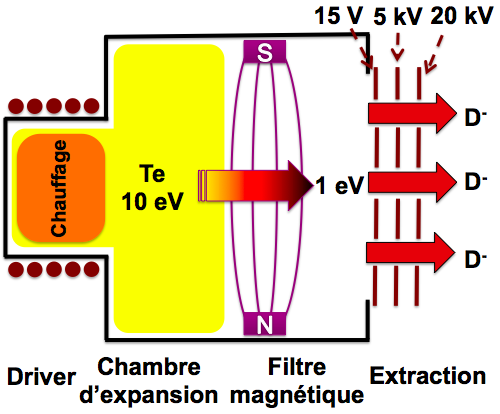
\includegraphics[height=5cm]{figures/sourceIPP.png}
    \caption{Schémas conceptuel du prototype de l'un des huits modules de la
    source IPP de Garching.
\label{4-GarchingSchema}}
\end{figure}

\begin{figure}[!htbp]
  \centering
    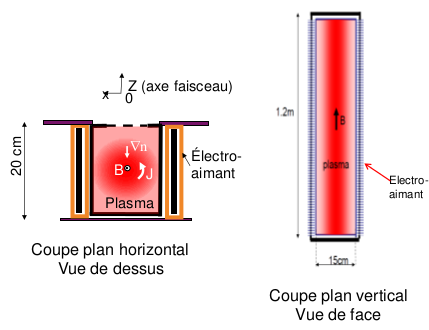
\includegraphics[height=8cm]{figures/4-cybeleSchema.png}
    \caption{Schémas de principe en coupe de Cybele~\parencite{SimoninHDR}. A
    gauche dans la vue de dessus, le champ magnétique est perpendiculaire au plan et confine le
plasma qui est créé au centre de la source. La vue de face montre quant-à elle
la fine colonne de plasma, de densité homogène sur toute sa hauteur.
\label{4-cybeleSchema}}
\end{figure}	

Actuellement, les sources d'ions négatifs en amont des IDN se servent d'un champ
magnétique en configuration filtre pour refroidir les électrons (un schéma de la
source développée pour ITER est rappelé sur la figure~\ref{4-GarchingSchema}).
Nous avons vu précédemment que cette configuration magnétique entraîne
dans ce type de sources de fortes inhomogénéités du plasma, avec l'émergence de
fort gradients de densité et de température dans le plan
perpenduculaire au champ~\parencite{Fantz,Kolev}.
L'uniformité du plasma généré par la source est cependant primordiale pour une
bonne efficacité de l'accélérateur dans l'IDN, et de nombreux efforts sont
portés pour palier à ce problème.

L'une des pistes étudiée est d'utiliser le champ magnétique non pas pour
filtrer les électrons énergétiques mais plutôt pour les confiner au centre
d'une colonne de plasma en rotation autour d'un axe magnétique (voir le schéma
de la figure~\ref{4-cybeleSchema}). Ce concept,
idéal pour la géométrie étirée de Cybele, permettrait d'obtenir une densité de
plasma homogène sur toute la longueur de la source. 

\subsection{Caractéristiques de la source}

La source Cybele est rectangulaire et de dimension 
15~cm x 20~cm x 120~cm. Le centre de la source est
occupé par des cathodes filamentaires qui, polarisées négativement à -60 V et
libèrent des électrons primaires de 70 eV
d'énergie pour créer et entretenir le plasma.
Celui-ci est ensuite confiné dans un champ magnétique vertical et uniforme, généré par deux
groupes de bobines\footnote{La décomposition des bobines
latérales sur la hauteur en plusieurs parties indépendantes permet de faire
varier l'intensité du champ magnétique localement. On peut ainsi créer une
configuration miroir pour retenir les électrons qui seraient sinon perdus très
rapidement le long de la direction parallèle. 

Une autre solution pour réduire
le transport parallèle des électrons consiste à polariser négativement les
parois aux extrémités des lignes de champ.} sur les côtés de la source,
l'intensité du champ pouvant varier de 0 G à 160 G. Cybele opère enfin avec un
gaz d'hydrogène à très basse pression, P $\simeq$ 0.7--2 mTorr, condition
requise pour réduire la perte des ions négatifs par le phénomène d'épluchage
électronique. Dans le cadre de la
ligne IDN Siphore, de rapport d'aspect laminaire, ce type de
source s'adapte parfaitement à l'accélérateur Singap (pour Single Aperture
Photo-neutralization) qui neutralise le faiseau d'ions négatif 
par photodétachement à l'aide d'un laser de 1 kW et d'une cavité de
Fabry-Perot~\parencite{SimoninHDR}.

Les mesures expérimentales en H$_2$, réalisées avec des sondes de
Langmuir~\parencite{Simonin}, donnent une densité d'environ 3.10$\puissance{18}$
m$\puissance{-3}$ au centre du plasma, et de 5.10$\puissance{17}$
m$\puissance{-3}$ en périphérie. La température électronique chute quant à
elle de 6 eV à un peu plus de 2 eV au niveau des parois latérales. Une mesure
temporelle du courant de saturation ionique (voir
figure~\ref{4-CybeleFourierSignal})  détecté la présence d'une
fluctuation périodique à une basse fréquence (un pic à 37kHz et une bande de largeur plus significative autour de 32kHz), signe éventuel d'un phénomène d'intermittence dans le plasma.

\begin{figure}[!htbp]
  \centering
    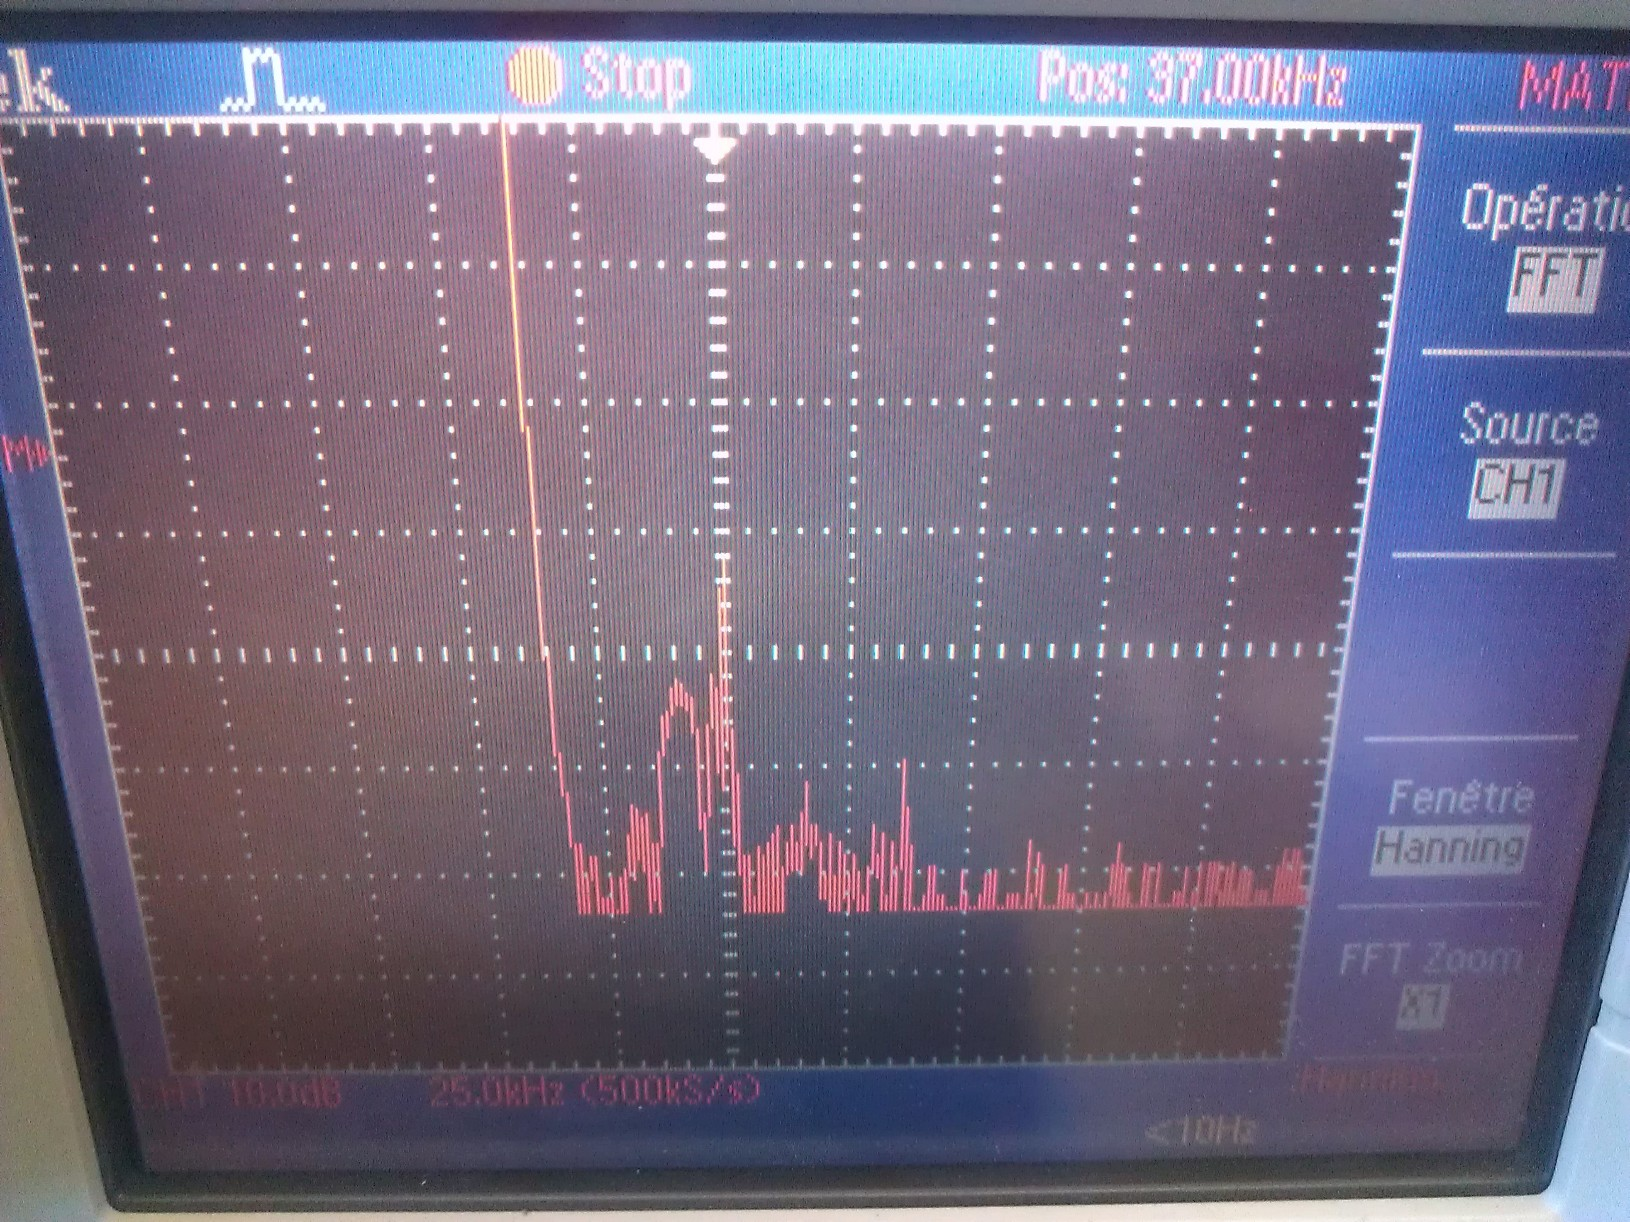
\includegraphics[height=6cm]{figures/4-CybeleFourierSignal.jpg}
    \caption{Spectre du courant de saturation
    ionique à r=5cm du centre de la source.
    L'oscilloscope est réglé sur 25kHz/carreau.\label{4-CybeleFourierSignal}}
\end{figure}

Là encore, une simulation concrète de l'évolution du plasma dans
Cybele nécessiterait la prise en compte des ions négatifs et de la source de
courant créée par le type de chauffage avec cathode émissive. L'étude qui suit
se limite à une colonne de plasma plus classique, telle que Mirabelle à
Nancy~\parencite{Mirabelle} ou NAGDIS-II au Japon~\parencite{NAGDIS1}.
 
\subsection{Simulation d'une colonne de plasma}

Dans une géométrie simple comme la colonne de plasma, avec un champ magnétique
axial et uniforme, de nombreuses tentatives ont été entreprises pour réduire le
problème multidimensionnel de diffusion du plasma à travers le champ à une
sorte de diffusion ambipolaire effective. Cependant, même à très faible champ
magnétique, la diffusion des ions et des électrons fondamentalement non
ambipolaire : les courants, qui se referment dans les parois aux extrémités des
lignes de champ et forment des vortex dans la direction perpendiculaire,
permettent de créer des phénomènes de court-circuit dans le plasma et stimulent
significativement le transport transverse~\parencite{Gurevich}.

Commençons par montrer les résultats d'une simulation classique. Le domaine de
simulation, sur la figure~\ref{4-cybeleSimDomain}, est pris de dimension
20x20x120 cm$\puissance{3}$ et représente toujours le plan transverse au champ
magnétique, qui est pris uniforme et d'intensité B=100G. Le plasma est créé au
centre du domaine par un chauffage de forme gaussienne en 2D, en supposant une
puissance absorbée d'environ 100W. La pression de gaz (Hydrogène) est fixée à
1mTorr avec toutes les parois conductrices et reliées à la masse (exceptées
celles aux extrémités les lignes de champ qui seront prises de nature isolante
dans un cas test.

\begin{figure}[!htbp]
\centering
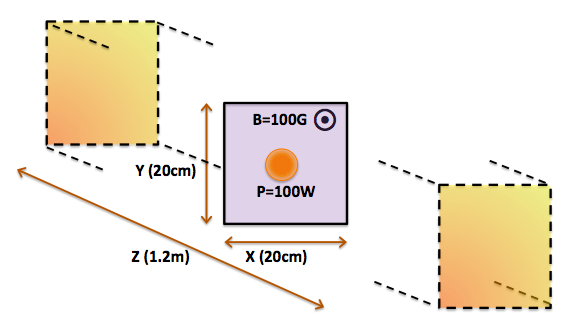
\includegraphics[width=0.8\textwidth]{figures/4-cybeleSimDomain.png}
{\caption{Le domaine de simulation est le plan perpendiculaire au champ
magnétique.}
\label{4-cybeleSimDomain}}
\end{figure}
\begin{figure}[!htbp]
  \centering
    \subfigure[]{\label{4-CybeleCarteDensiteBase}
    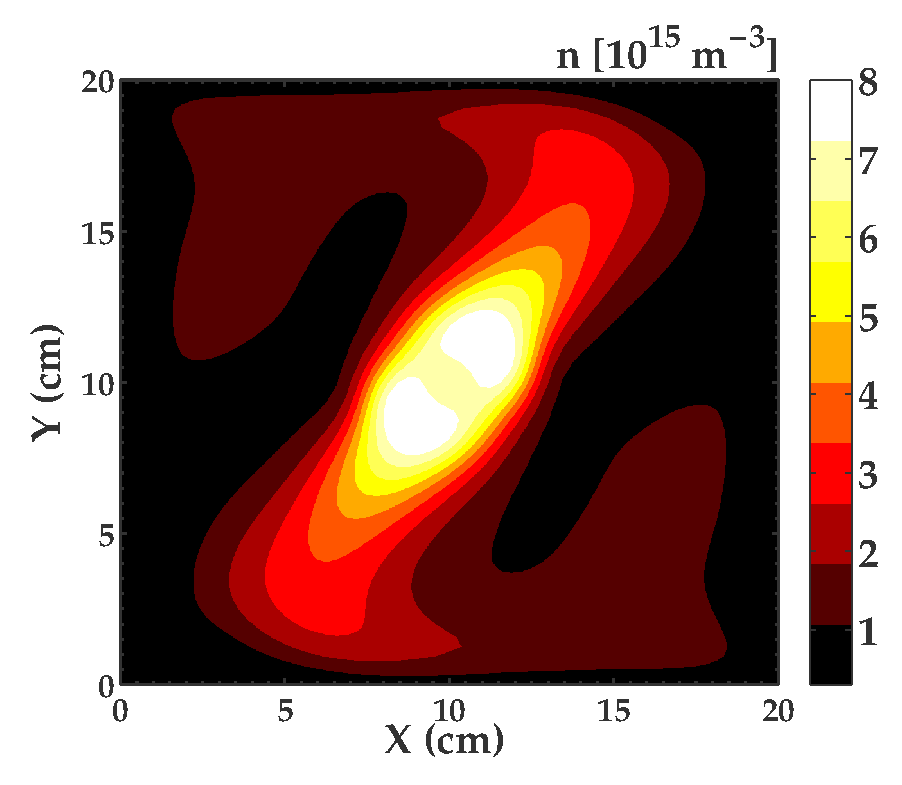
\includegraphics[height=5.5cm]{figures/4-CybeleCarteDensiteBase.eps}}
    \subfigure[]{\label{4-CybeleCartePotentielBase}
    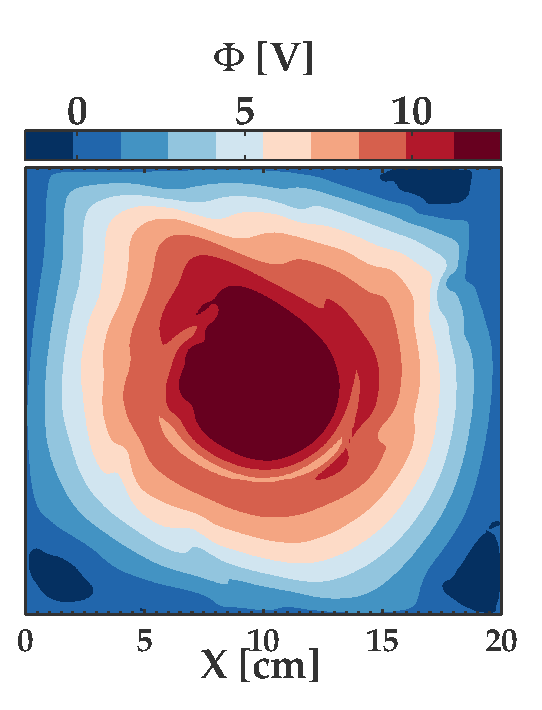
\includegraphics[height=5.5cm]{figures/4-CybeleCartePotentielBase.eps}}
    \subfigure[]{\label{4-CybeleCarteTemperatureBase}
    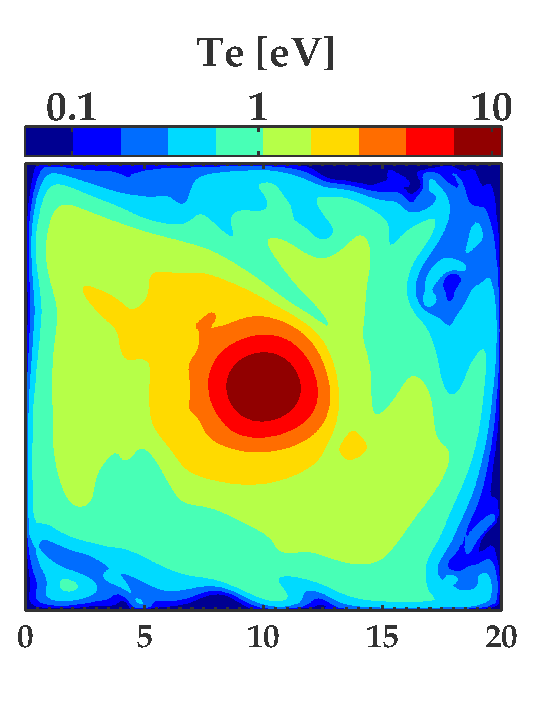
\includegraphics[height=5.5cm]{figures/4-CybeleCarteTemperatureBase.eps}}
    \caption{Cartes de densité \subref{4-CybeleCarteDensiteBase}~, de
    potentiel \subref{4-CybeleCartePotentielBase}~ et de
    température \subref{4-CybeleCarteTemperatureBase}}
    \label{CybeleCartesBase}
\end{figure}

Les solutions obtenues par MAGNIS avec ces paramètres sont illustrées
figure~\ref{CybeleCartesBase}. La densité est maximale\footnote{La
densité maximale du plasma est directement contrôlée par la puissance
absorbée. Bien que celle-ci soit de deux ordres de grandeur inférieure à la
densité mesurée dans Cybele, il suffit de choisir une puissance absorbée
cohérente pour obtenir un résultat proche des mesures expérimentales.} au centre
de la source à 3.10$\puissance{16}$ m$\puissance{-3}$, et
exponentiellement décroissante sur une longueur de 2 à 3 cm. Le phénomène le plus
remarquable est cependant la formation d'un bras de plasma (ou un long filament
en 3D) partant de la zone centrale et tournant à une vitesse angulaire
constante.
Une rotation complète de cette structure de mode $m=$1 s'effectue en $T\simeq$
23 \micro s, correspondant à une vitesse angulaire de :

\begin{equation}
\Omega_R=\frac{2\pi m}{T}\simeq2.25\;10^5\text{rad/s}
\end{equation}

Les images enregistrées avec une caméra rapide lors des expérimentations
sur NAGDIS-II (voir figure~\ref{4-CybeleNagdis}) ont déjà montré un comportement
similaire du plasma, ce qui est là aussi très
encourageant sur la validité des solutions trouvées par MAGNIS. Le potentiel
décroît monotonement de 12V à un peu moins de 0V dans la direction radiale et
ne rend que faiblement compte de la structure de densité.
 La température présente quant-à elle un fort gradient, passant de 10 eV à moins
 d'1 eV sur 2 à 3 cm de longueur.

\begin{figure}[!htbp]
\centering
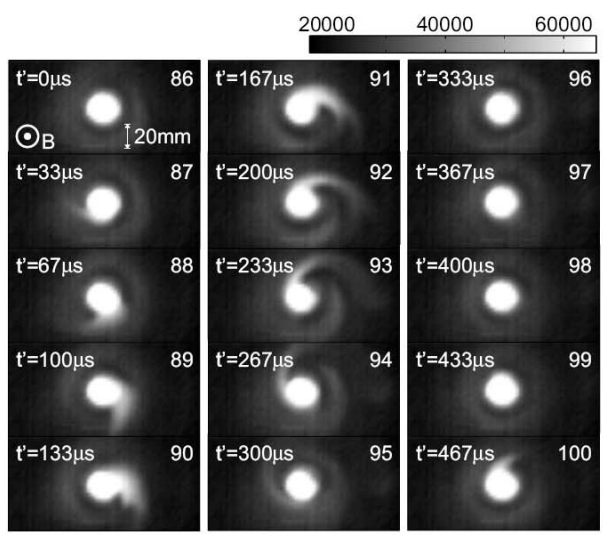
\includegraphics[width=0.5\textwidth]{figures/4-CybeleNAGDIS.png}
\caption{Images successives prises par caméra rapide~\parencite{NagdisCamera}.
La structure effectue une rotation complète en 230 \micro s et apparaît par
intermittence.
\label{4-CybeleNagdis}}
\end{figure}

Dans les colonnes de plasma magnétisées, les électrons ont tendance à s'échapper
le long des lignes de champ dans la direction parallèle. Le flux électronique
est alors déterminé par les conditions de gaine de Bohm~\parencite{Stangeby} et
entièrement gouverné par le rapport $\Phi/T_e$. Au centre du plasma, la
température électronique est très élevée. Pour retenir les électrons, le
potentiel plasma augmente, atteignant un ratio $\Phi/T_e$ de 1.1515 permettant
de déduire une densité de courant parallèle négative de :
\begin{equation}
\mathbf j_\para=enc_s(1-\exp(\Lambda-1.1515))\sim -600\text{A.m}\puissance{-2}
\end{equation}

qui est une estimation assez correcte de la valeur résolue par le modèle (-780
A.m$\puissance{-2}$). En dehors du plasma central, le ratio devient supérieur
au potentiel flottant, inversant le signe du courant récupéré au bout les lignes
de champ. Les électrons sont accélérés afin de compenser la trop grande perte de
charges positives. On peut placer la frontière entre ces deux régions au niveau
de la fin du plasma central, indiquant une modification dans le transport des
particules à cet endroit.

La figure~\ref{4-CybeleProfilsRadial} montre le profil radial moyennés dans le
temps des précédents champs, du centre de la source au bord X=20cm. Le plasma
est confiné sur un rayon de 4 cm tandis que le potentiel plasma
diminue progressivement, bien que de façon un peu plus prononcée juste après la
chute de densité du plasma. 
Le profil poloïdal est moyenné sur un repère tournant, qui positionne le pic de
densité en $\theta=-\pi/2$. On peut remarquer la présence d'une légère avance de
phase de la température sur la densité. Le potentiel, de son côté, est de forme
sinusoïdale et montre aussi un déphasage, dans le sens opposé, avec la densité.

\begin{figure}[!htbp]
  \centering
    \subfigure[]{\label{4-CybeleProfilsRadial}
    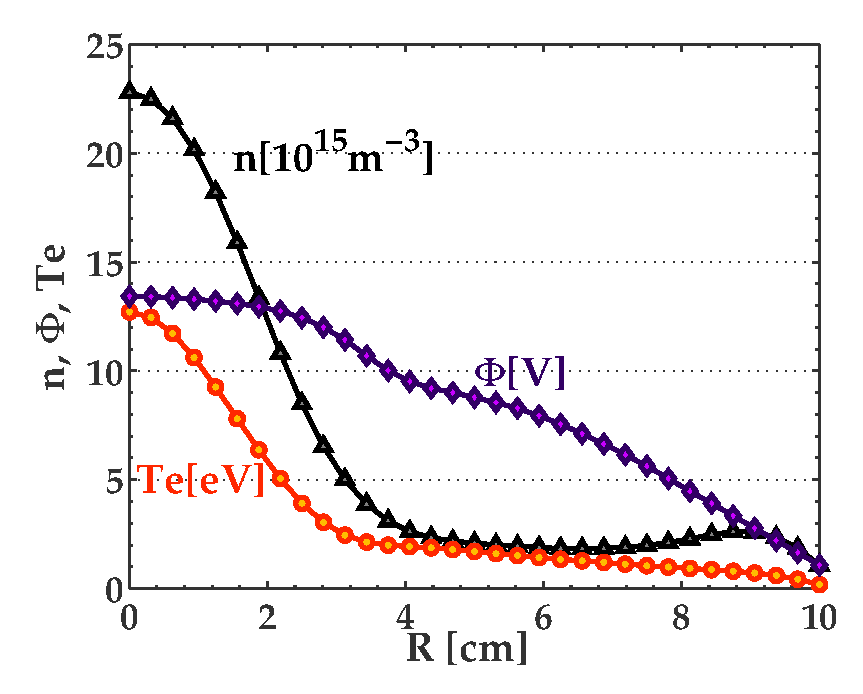
\includegraphics[height=5.2cm]{figures/4-CybeleProfileTempRadiale.eps}}
    \subfigure[]{\label{4-CybeleProfilsPol}
    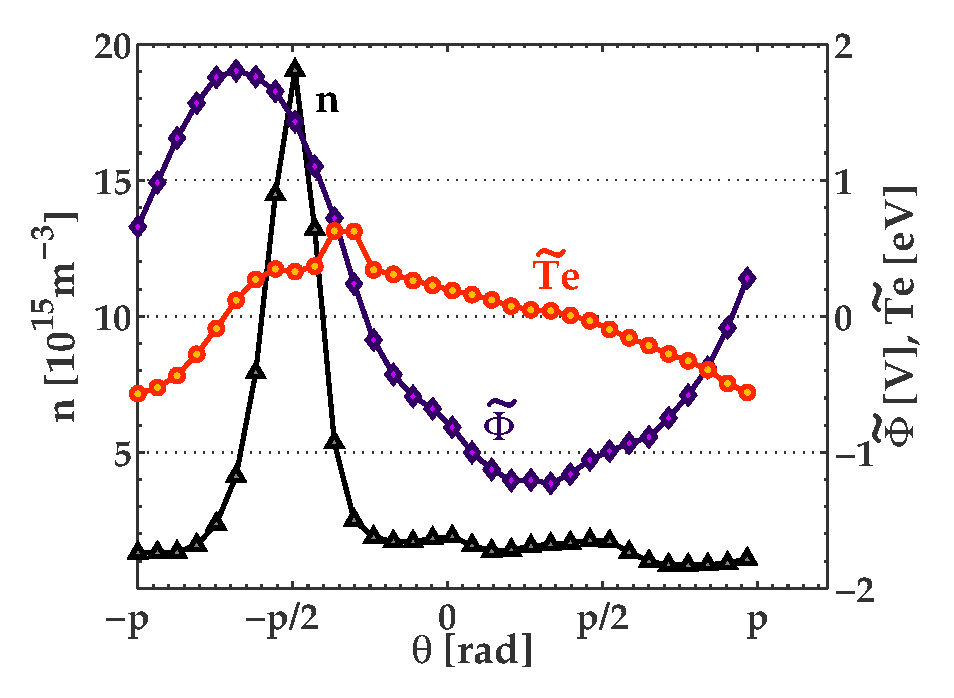
\includegraphics[height=5.2cm]{figures/4-CybeleProfileTempPol.eps}}
    \caption{Profils radiaux~\subref{4-CybeleProfilsRadial}~ et
    poloïdaux~\subref{4-CybeleProfilsPol}~ moyennés en temps de la densité, du
    potentiel et de la température. Le profil radial est pris du centre de la source au bord droit
    en X=20cm. Le profil poloïdal est moyenné sur un repère tournant qui suit
    la structure de densité à r=5 cm du centre de la source. Les quantités
    $\tilde{\Phi}$ et $\tilde{T}_e$ sont les variations de potentiel et de température par rapport à leur valeur
    moyenne, qui sont respectivement égale à 9V et 2eV. La structure se déplace
    dans le sens horaire, ie. vers les $\theta$ croissants.}
    \label{4-CybeleProfils}
\end{figure}

Pour déterminer l'origine de la structure et de la rotation, intéressons nous
tout d'abord aux flux électronique et ionique dans la direction
transverse, illustrés sur la figure~\ref{4-CybeleCarteFlux}.
Les ions, créés au centre de la source, traversent le champ magnétiques et
tombent aux parois en effectuant des spirales dans le même sens que le bras de
densité. On constate que le courant ionique est maximal au centre de la source,
et qu'un fort flux passe par la surdensité. La vitesse du fluide ionique
est cependant deux à trois fois moins importante que la vitesse de rotation de
la structure. Sur la seconde image, on peut remarquer que le fluide électronique
change de direction après un minimum, situé là encore aux alentours de la
frontière du plasma confiné.

\begin{figure}[!htbp]
  \centering
    \subfigure[]{\label{4-CybeleCarteFluxIBase}
    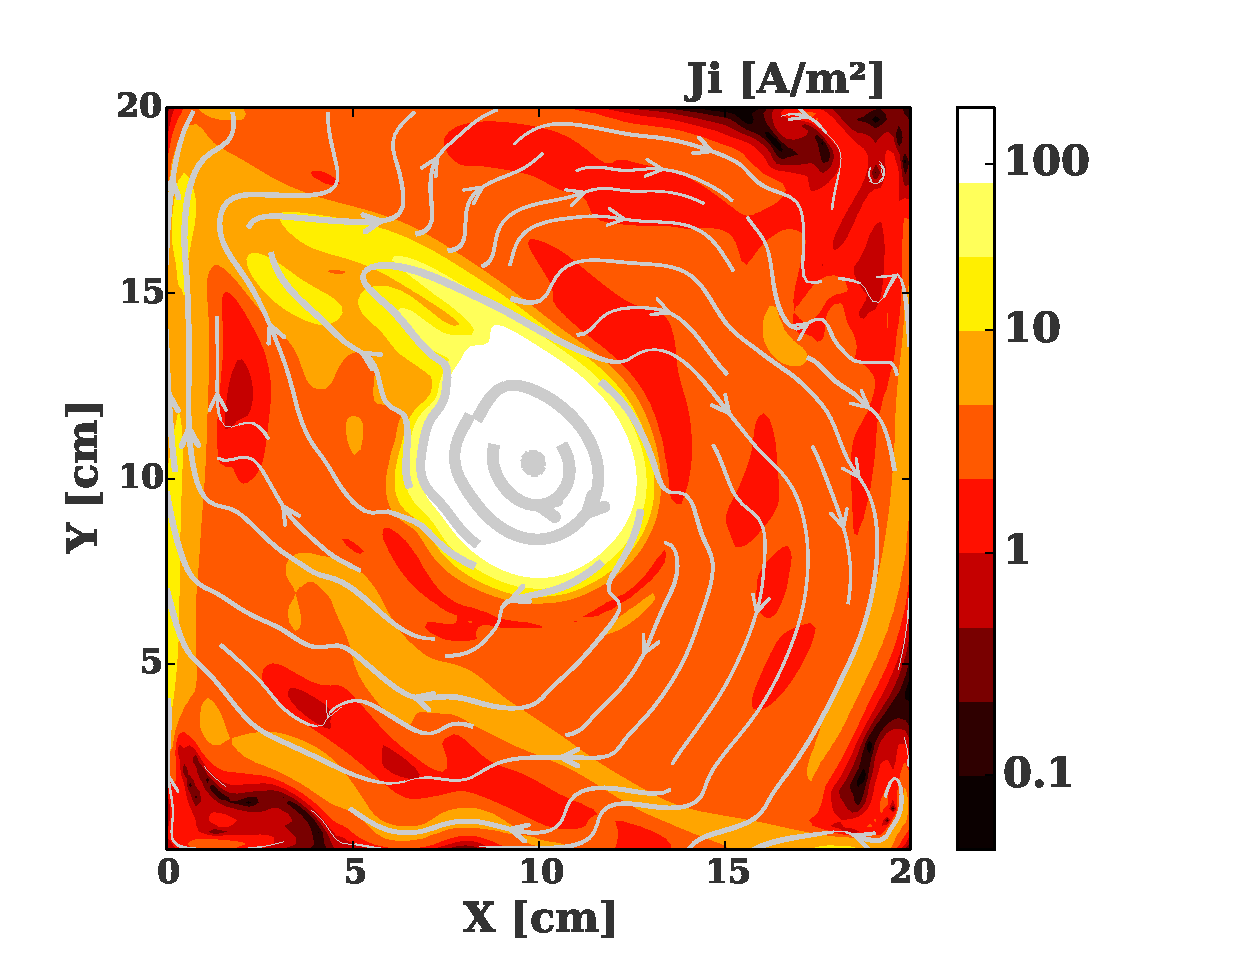
\includegraphics[height=5.5cm]{figures/4-CybeleCarteFluxIBase.eps}}
    \subfigure[]{\label{4-CybeleCarteFluxEBase}
    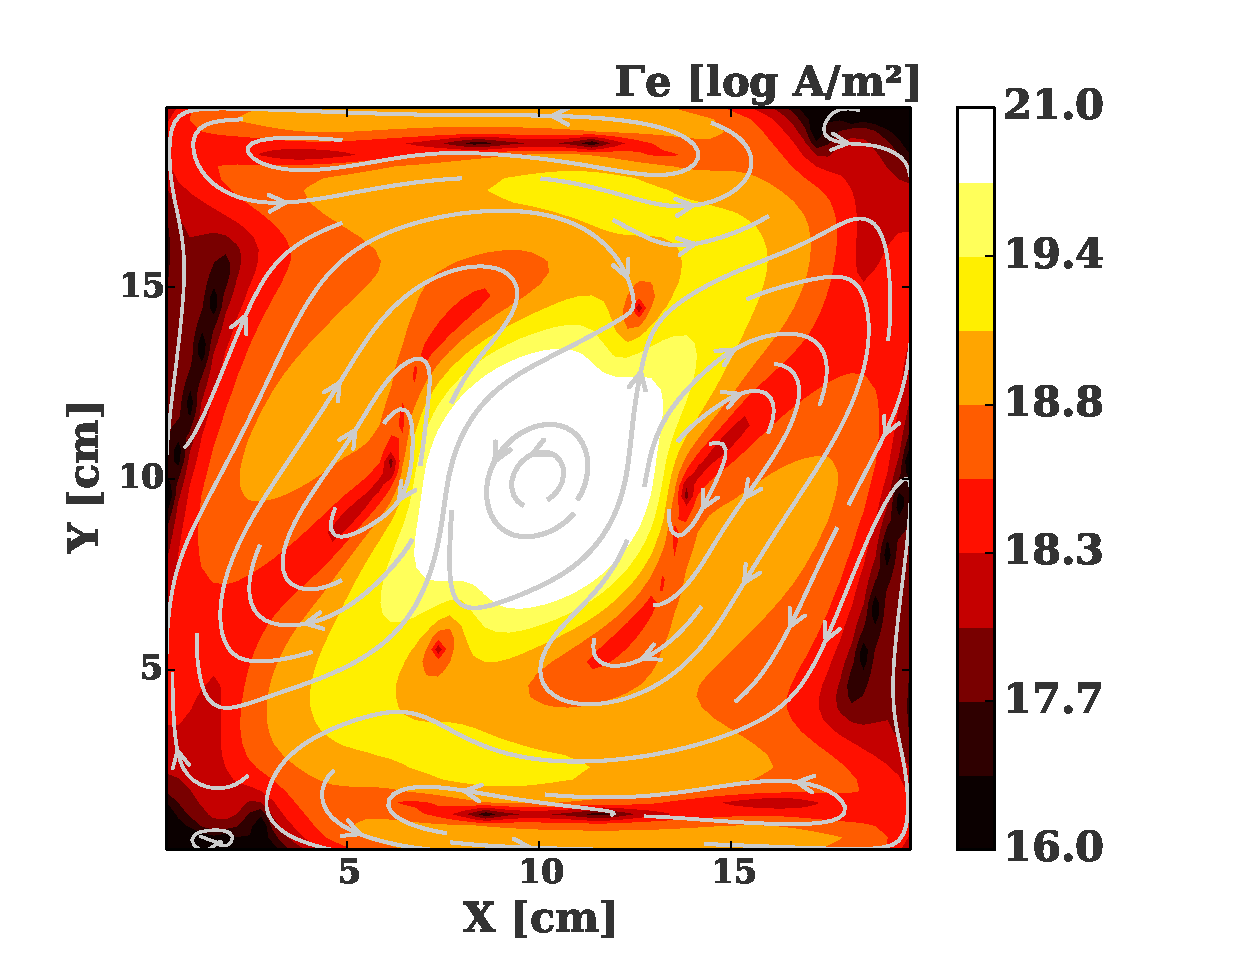
\includegraphics[height=5.5cm]{figures/4-CybeleCarteFluxEBase.eps}}
    \caption{Cartes de densité \subref{4-CybeleCarteFluxEBase}~ et de
    température \subref{4-CybeleCarteCourant}}
    \label{4-CybeleCarteFlux}
\end{figure}

Dans la direction radiale et en présence d'un champ magnétique, les gradients
moyens de potentiel et de pression donnent naissance à une vitesse de dérive
fluide. Le champ électrique radial moyen $E_r$ d'environ 120 V/m, entraîne
théoriquement une dérive poloïdale de l'ordre de :
\begin{equation}
\omega_E=\frac{E_r}{rB}\simeq10^5\,\text{rad/s} 
\end{equation}
qui est du même ordre de grandeur que la vitesse de rotation du bras de plasma.
La figure~\ref{4-CybeleVitessesDerive} montre les profils de ces deux vitesses
de dérive le long de la direction radiale. On observe que la vitesse de dérive
diamagnétique, ie. liée au gradient de pression, est dominante au centre du
plasma. 

\begin{figure}[!htbp]
\centering
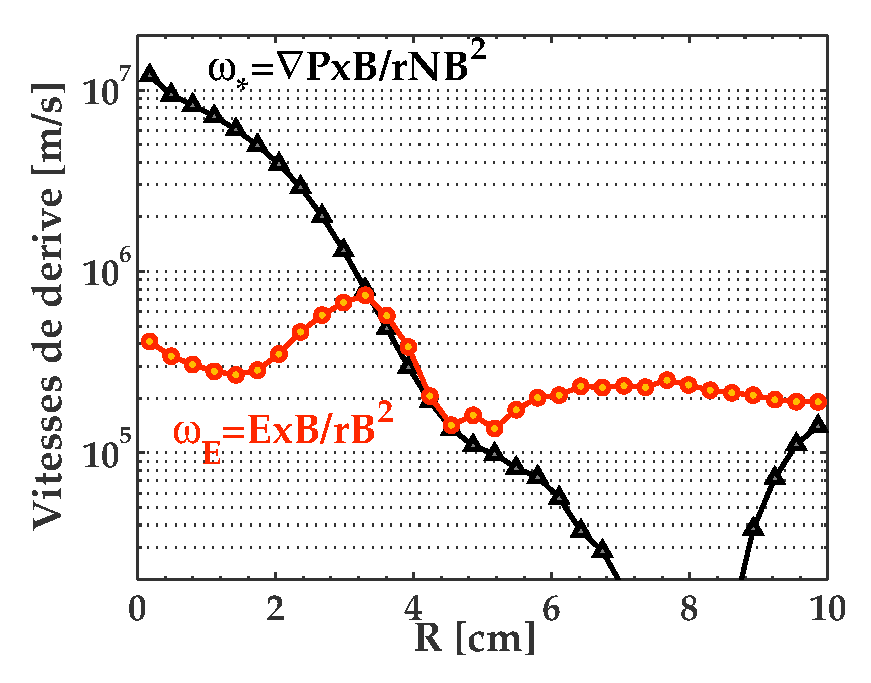
\includegraphics[width=0.5\textwidth]{figures/4-CybeleProfileVitessesDerive.eps}
{\caption{Carte de densité à 35G.}
\label{4-CybeleVitessesDerive}}
\end{figure}

Cette dérive entraîne les ions et les électrons dans des directions
contraires, générant un fort courant. A r~$\sim$~4~cm, au niveau de la
séparation, les deux vitesses s'égalisent, puis la vitesse de dérive électrique, qui ne
génère que peu de courant, prend le dessus. Dans la région traversée par le bras
de densité, $\omega_E\simeq$ 2,3.10$\puissance{6}\,\text{rad.s}\puissance{-1}$
est très proche de la vitesse de rotation mesurée.

Lors de l'exploration des modes de fonctionnement de la source, le transport
dans la colonne de plasma s'est révélé principalement sensible à deux
paramètres : L'intensité du champ magnétique et les conditions parallèles 
(longueur de la source et nature des parois). Les deux sections suivantes
montrent un rapide aperçu de l'influence de ces variables.

\subsection{Variation croissante du champ magnétique}
Nous reprenons dans cette partie les conditions de base utilisées précédemment.
En l'absence de champ magnétique, le transport est isotrope. La différence de
mobilité entre les ions et les électrons donne naissance à un champ électrique
dit ambipolaire qui les fait dériver ensemble jusqu'aux parois. Le plasma
d'hydrogène a une densité de 3.10$\puissance{14}$ m$\puissance{-3}$ et sa
température, assez homogène, est de 11eV. Ajoutons maintenant un champ
magnétique : au fur et à mesure de la montée en intensité, on peut repérer 4
modes de fonctionnement.

\subsubsection{de 0G à 2G}

\begin{figure}[!htbp]
  \centering
    \subfigure[]{\label{4-CybeleVarMag1}
    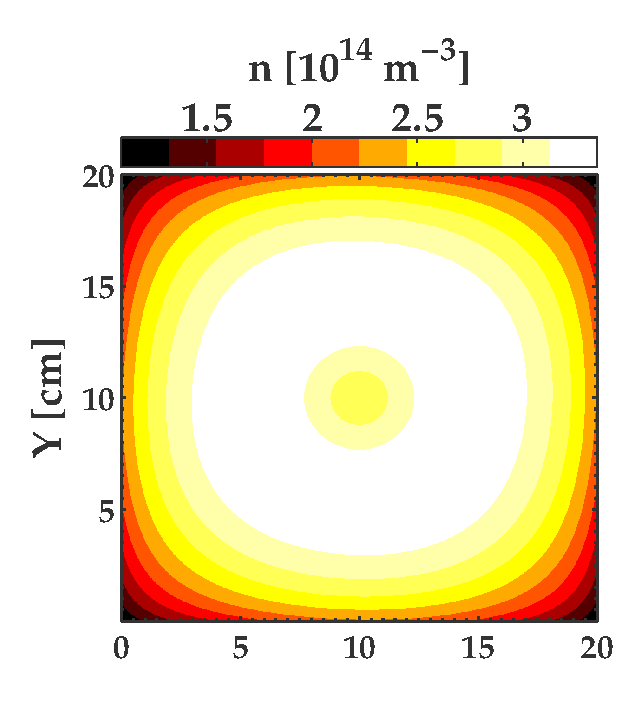
\includegraphics[height=5.5cm]{figures/4-CybeleVarMag1.eps}}
    \subfigure[]{\label{4-CybeleVarMag2}
    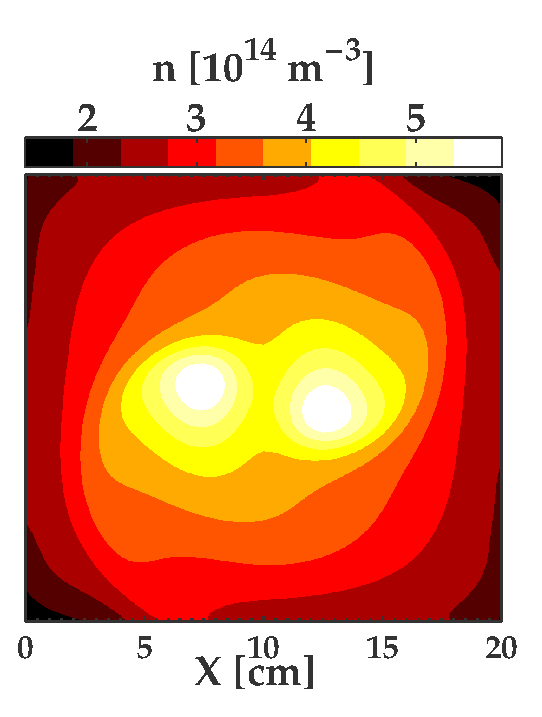
\includegraphics[height=5.5cm]{figures/4-CybeleVarMag2.eps}}
    \subfigure[]{\label{4-CybeleVarMag3}
    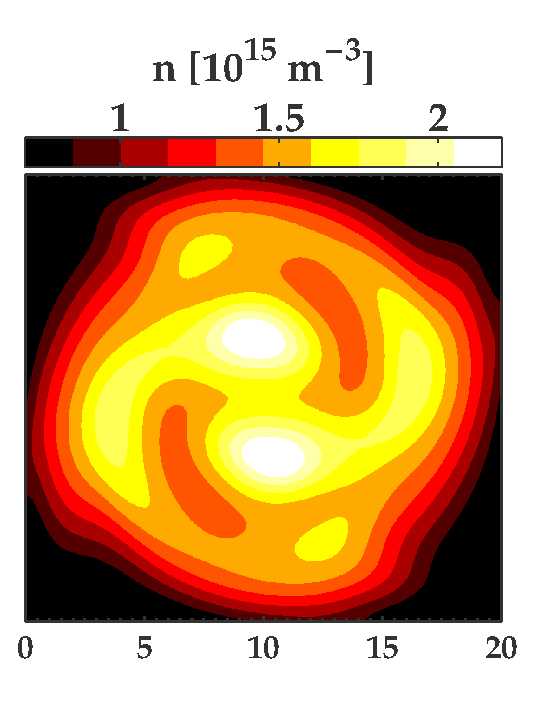
\includegraphics[height=5.5cm]{figures/4-CybeleVarMag3.eps}}
    \caption{Cartes de densité à 1G\subref{4-CybeleVarMag1}~, 4G
    \subref{4-CybeleVarMag2}~ et 15G \subref{4-CybeleVarMag3}}
    \label{4-CybeleVarMag-1}
\end{figure}

L'apparition d'un faible champ magnétique modifie légèrement la nature du
transport. Observons la figure~\ref{4-CybeleVarMag1} : entre 1 G et 2 G, le
plasma forme un anneau, de densité équivalente au cas non
magnétisé. La température au centre de la source s'élève, passant 
successivement à 14 eV puis à 20 eV. Le rayon de l'anneau est approximativement
égal au rayon de Larmor électronique local, qui s'encadre par :
\begin{equation}
\frac{L_\perp}{2}=10\,\text{cm}>\rho\indice{e}>l_c\simeq 5\,\text{cm}
\end{equation}
où $L_\perp$ est la longueur caractéristique de la source et $l_c$ une distance
critique. 

\subsubsection{de 3G à 15G}
A partir de 3G, le plasma se met en rotation, changeant encore de forme (comme
le montre la figure~\ref{4-CybeleVarMag2}). Deux îlots de densité plus élevée
apparaissent, tournant à une vitesse angulaire $\Omega_r$ qui varie de 1 à 
2.10$\puissance{6}\,\text{rad.s}\puissance{-1}$ sur une orbite de rayon
 approximativement égale au rayon de Larmor électronique, qui devient inférieur
à 5cm. La température maximale commence à osciller\footnote{A B=7.5G, la
fréquence cyclotronique électronique est égale à
1,3.10$\puissance{8}\,\text{s}\puissance{-1}$, très proche de la fréquence de
collision des électrons. Le maximum de température atteint son plus haut taux de fluctuation.} et augmente plus modérément.

Ce type de fonctionnement, qui est caractérisé par une
fréquence de rotation assez rapide et la présence d'une structure de densité de
mode m=2, se manifeste jusqu'à un champ magnétique d'une petite vingtaine de
gauss. 

\subsubsection{de 18G à 70G}
Entre 18G et 30G, le plasma devient extrêmement instable, comme illustré
sur la figure~\ref{4-CybeleVarMag-2} : le plasma croît en
densité et en température jusqu'à atteindre une valeur critique, puis relaxe
très rapidement en créant une onde de surdensité. La fréquence de ce cycle
est d'environ 9~kHz.
\begin{figure}[htbp]
  \centering
    \subfigure[]{\label{4-CybeleVarMag4}
    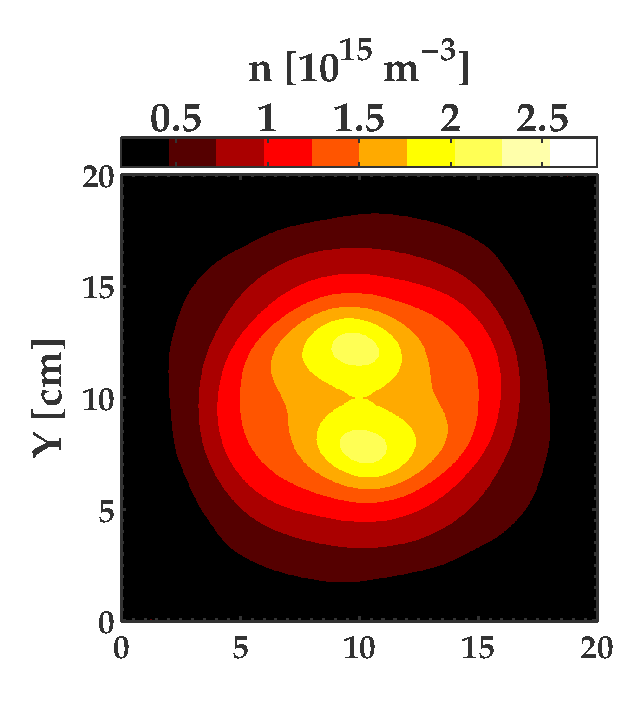
\includegraphics[height=5.5cm]{figures/4-CybeleVarMag4.eps}}
    \subfigure[]{\label{4-CybeleVarMag5}
    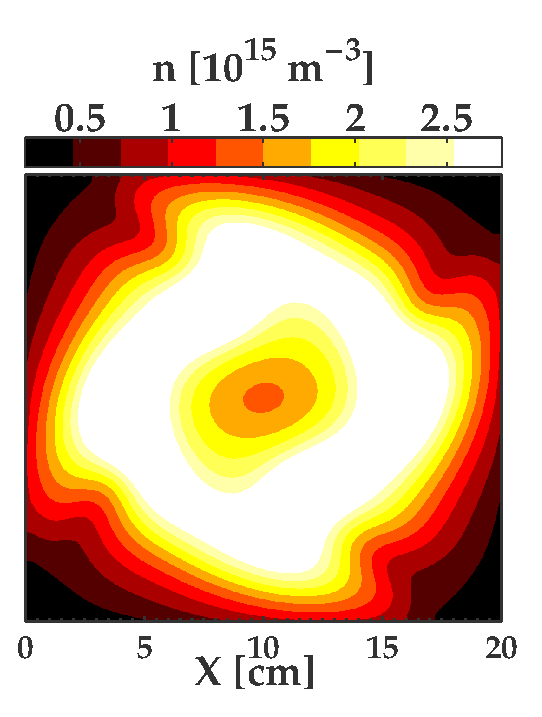
\includegraphics[height=5.5cm]{figures/4-CybeleVarMag5.eps}}
    \subfigure[]{\label{4-CybeleVarMag6}
    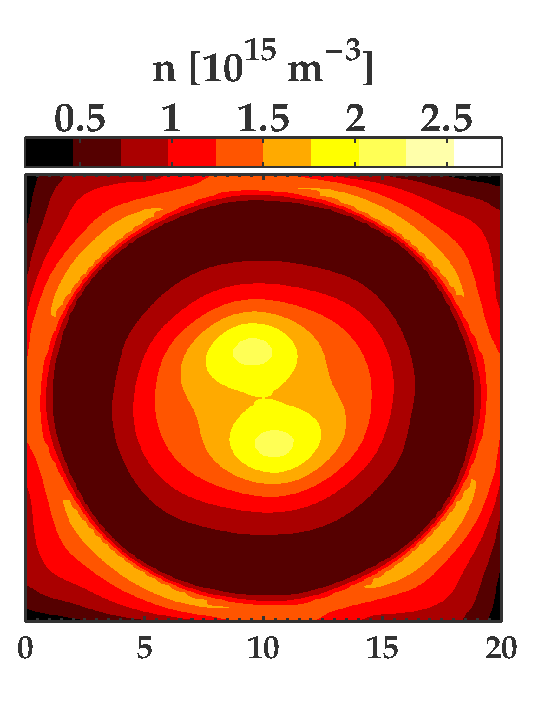
\includegraphics[height=5.5cm]{figures/4-CybeleVarMag6.eps}}
    \caption{Cartes de densité à 20G à trois instants
    différents.}
    \label{4-CybeleVarMag-2}
\end{figure}
La figure~\ref{4-CybeleVarMag8} montre la forme du plasma à 35G, qui s'est
stabilisé. La température moyenne des électrons redescend à une quinzaine
d'électronvolts, faisant diminuant le rayon de Larmor ionique jusqu'à une
longueur de l'ordre de la dizaine de centimètres, soit une longueur inférieure à
la longueur caractéristique du système.
Plusieurs pics, situés à la frontière du plasma, sont de densités 2 à 3 fois
supérieure à la densité centrale. On commence aussi à voir apparaître un bras en
périphérie du plasma, qui tourne à une fréquence de 50kHz. 
\begin{figure}[!htbp]
\centering
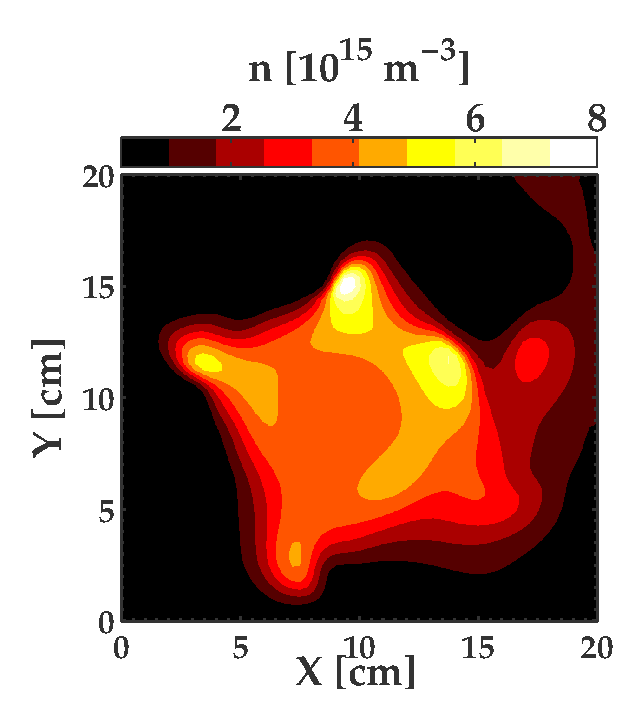
\includegraphics[width=0.33\textwidth]{figures/4-CybeleVarMag8.eps}
{\caption{Carte de densité à 35G.}
\label{4-CybeleVarMag8}}
\end{figure}

De 35G à 70G, le plasma est dans un régime transitoire : la température
et la densité oscillent fortement, et les surdensités sont relaxées à travers 
le mode poloïdal qui se développe de plus en plus.
\subsubsection{de 70G à 170G}
A partir de 70G, le rayon de Larmor ionique devient inférieur à 5cm : les ions
peuvent être considérés comme magnétisés.
Sur la figure~\ref{4-CybeleVarMag9}, on voit que le
plasma forme une spirale. La structure poloïdale de mode m=1 tourne à une
vitesse de 4.10$\puissance{5}\,\text{rad.s}\puissance{-1}$. Les
figures~\ref{4-CybeleVarMag10} et~\ref{4-CybeleVarMag11} représentent la densité
du plasma à 130G (où le plasma se déplace en effectuant une rotation presque
solide) et 170G, caractérisée par l'apparition d'un mode poloïdal m=2. 
Le tableau~\ref{4-CybeleVarMagTab} résume les propriétés du plasma observées
dans cette partie.
\begin{figure}[!htbp]
  \centering
    \subfigure[]{\label{4-CybeleVarMag9}
    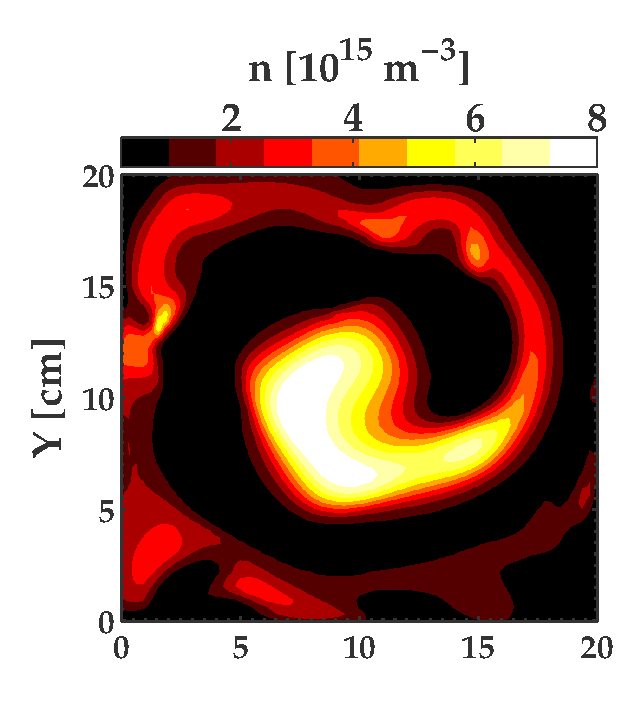
\includegraphics[height=5.5cm]{figures/4-CybeleVarMag9.eps}}
    \subfigure[]{\label{4-CybeleVarMag10}
    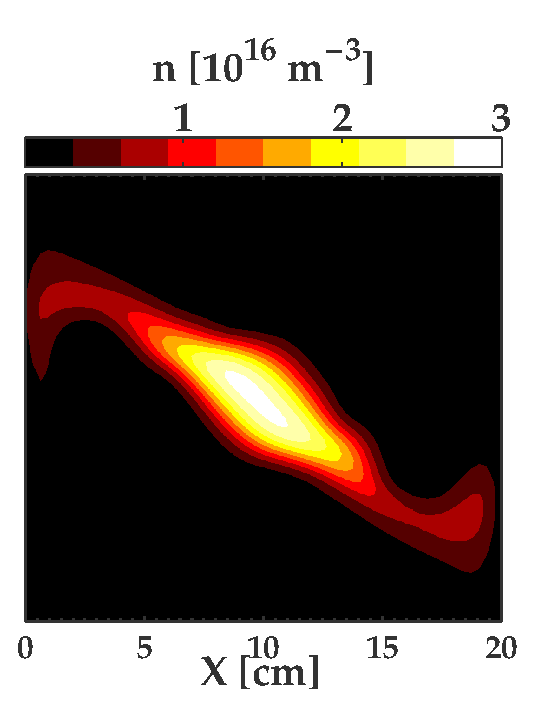
\includegraphics[height=5.5cm]{figures/4-CybeleVarMag10.eps}}
    \subfigure[]{\label{4-CybeleVarMag11}
    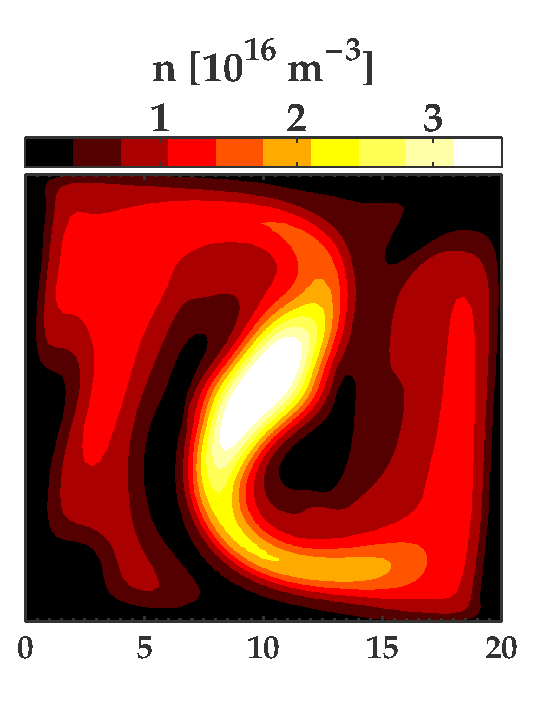
\includegraphics[height=5.5cm]{figures/4-CybeleVarMag11.eps}}
    \caption{Cartes de densité à 80G~\subref{4-CybeleVarMag9}~, 130G
    \subref{4-CybeleVarMag10}~ et 170G \subref{4-CybeleVarMag11}}
    \label{4-CybeleVarMag-3}
\end{figure}


\begin{table*}
\footnotesize\centering
\ra{1.3}
\begin{tabular}{@{}ccccccccc@{}}\toprule
B&&\multicolumn{2}{c}{Champs}&&\multicolumn{2}{c}{Échelles} &&
Rotation\\
\cmidrule{3-4} \cmidrule{6-7} \cmidrule{9-9}
&& $n$ (m\textsuperscript{-3}) & $T_e$ (eV)&& $\omega_\alpha$
&$\rho\indice{\alpha}$&& $\Omega_r$ (10\textsuperscript{5}rad/s)\\
\midrule Phase 1&&&&&\multicolumn{2}{c}{électrons}\\
\scriptsize 1-2 &&\scriptsize 3.3 10\textsuperscript{14} $\nearrow$~~
\scriptsize 3.5 10\textsuperscript{14} &\scriptsize14 $\nearrow$~~\scriptsize 20 &&
$\omega_e<\nu_e$ &\scriptsize$\rho\indice{e}\sim L_\perp$ && \scriptsize -
\\
Phase 2\\
\scriptsize 3-15 &&\scriptsize 5.5 10\textsuperscript{14}
$\nearrow$~~\scriptsize 1.8 10\textsuperscript{15} &\scriptsize22
$\nearrow$~~\scriptsize 28.5 && $\omega_e\sim\nu_e$ &\scriptsize$\rho\indice{e}<
L_\perp$ && \scriptsize 10 $\nearrow$~~\scriptsize20
\\
Phase 3 &&&&&\multicolumn{2}{c}{ions}\\
\scriptsize 17-60 &&\scriptsize 2 10\textsuperscript{15} $\nearrow$~~\scriptsize
2 10\textsuperscript{16} &\scriptsize$\in$ \scriptsize [26 - \scriptsize 37]
&& $\omega_i<\nu_i$ &\scriptsize$\rho\indice{i}\sim L_\perp$ && \scriptsize N.A.
\\
Phase 4 \\
\scriptsize 70-170 &&\scriptsize 1.3 10\textsuperscript{16}
$\nearrow$~~\scriptsize 4.5 10\textsuperscript{16} &\scriptsize23
$\searrow$~~\scriptsize 9 && $\omega_i\sim\nu_i$ &\scriptsize$\rho\indice{i}<
L_\perp$ && \scriptsize 4 $\searrow$~~\scriptsize1.5$\nearrow$~~\scriptsize2
\\
\bottomrule
\end{tabular}
\caption{Tableau résumant les principales
caractéristiques de la colonne de plasma dans un champ
magnétique variant de 1G à 170G.}\label{4-CybeleVarMagTab}
\end{table*}

Cette étude sur la variation croissante du champ magnétique montre tout d'abord
que le plasma se comporte très différemment en fonction des diverses plages
d'intensité, avec parfois la superposition de plusieurs types de transport.
Ensuite nous pouvons constater que globalement, la densité augmente en fonction
du champ magnétique tandis que la température électronique progresse tout
d'abord jusqu'à une trentaine d'eV, puis redescend sous la barre des 10eV. 

Enfin on note qu'un mode poloïdal se développe en
présence du champ magnétique, avec un unique bras tournant à une
vitesse angulaire $\Omega_r\sim$ 2.3 10\textsuperscript{5} rad/s. Dans
certaines conditions un deuxième bras peut aussi apparaître, de vitesse
inférieure au premier - ou égale auquel cas les deux bras tournent en phase de
part et d'autre du centre de la source.

\subsection{Rôle de la direction parallèle}

\begin{figure}[!htbp]
  \centering
    \subfigure[]{\label{4-CybeleProfileDenRadialeZ}
    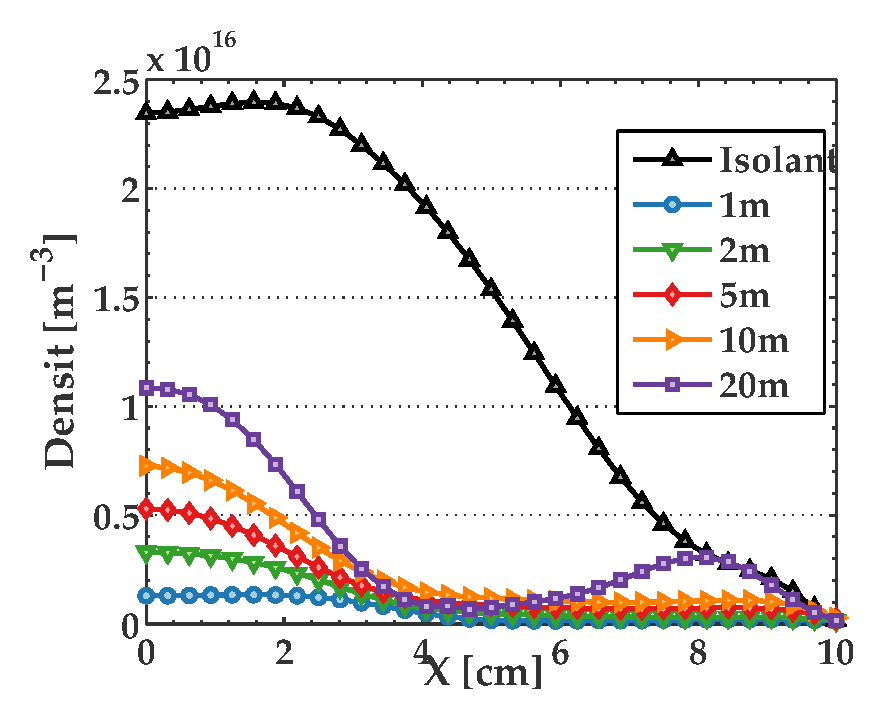
\includegraphics[height=5.25cm]{figures/4-CybeleProfileDenRadialeZ.eps}}
    \subfigure[]{\label{4-CybeleProfileTempRadialeZ}
    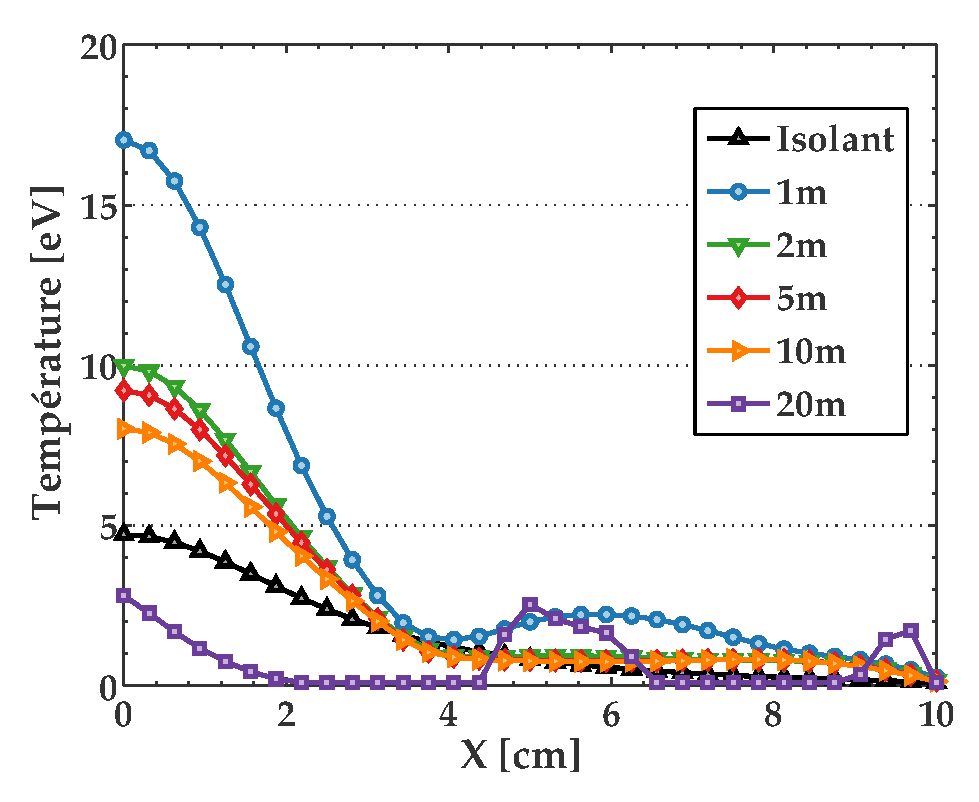
\includegraphics[height=5cm]{figures/4-CybeleProfileTempRadialeZ.eps}}
    \caption{Comparaison des profils de
    densité~\subref{4-CybeleProfileDenRadialeZ}~ et de
    température~\subref{4-CybeleProfileTempRadialeZ}~ pour différentes
    longueurs parallèles}
    \label{4-CybeleProfileDenRadiale}
\end{figure}

La direction parallèle joue aussi un rôle très influent dans la
dynamique du plasma. En laissant plus ou moins la possibilité aux électrons (et
donc au courant) de sortir du système par les parois, les contraintes imposées
au transport transverse évoluent. La figure~\ref{4-CybeleProfileDenRadiale}
montre les profils radiaux de densité et de température pour différentes
longueurs de source ainsi qu'un cas dans lequel les parois aux extrémités des lignes de champ
sont choisies isolantes. En toute généralité, on peut constater que l'effet
principal de l'augmentation de la longueur parallèle est de faire monter la
densité tout en abaissant la température.
L'allongement de la source a le même effet que l'augmentation de l'intensité du
champ magnétique, ie. on voit sur la densité une structure poloïdale de mode
m=1, voir m=2 à certaines longueurs.

La figure~\ref{CybeleCartesIsolant} montre les différents champs dans le cas de
parois isolantes. Le plasma, qui ne peut plus s'échapper le long de la direction
parallèle, s'étire dans la direction transverse tandis que la rotation se
saccade.
Le champ électrique et la température dans le plasma sont très faibles, et on
peut observer un anneau s'étalant sur toute la largeur de la source où le
potentiel est un peu plus bas.

\begin{figure}[!htbp]
  \centering
    \subfigure[]{\label{4-CybeleCarteDensiteIsolant}
    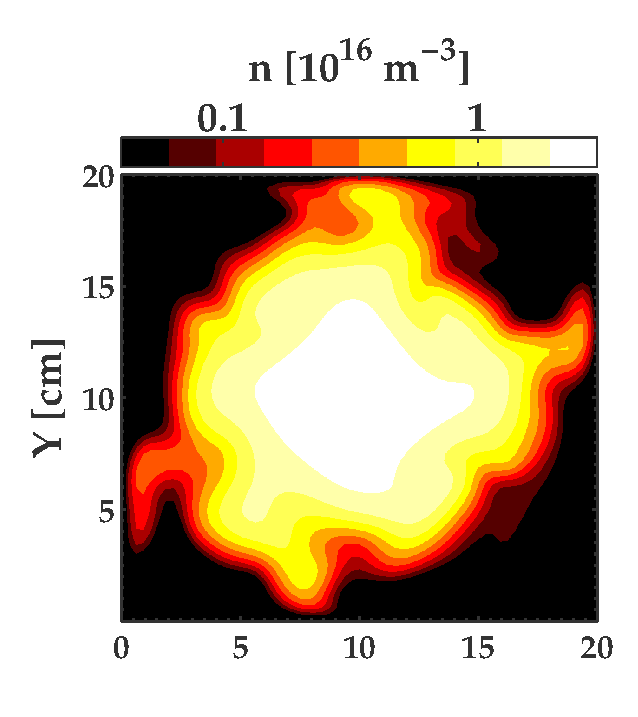
\includegraphics[height=5.5cm]{figures/4-CybeleCarteDensiteIsolant.eps}}
    \subfigure[]{\label{4-CybeleCartePotentielIsolant}
    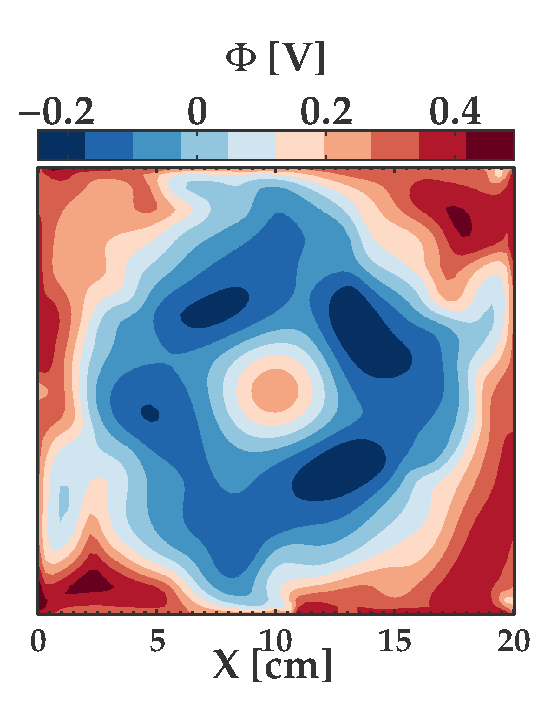
\includegraphics[height=5.5cm]{figures/4-CybeleCartePotentielIsolant.eps}}
    \subfigure[]{\label{4-CybeleCarteTemperatureIsolant}
    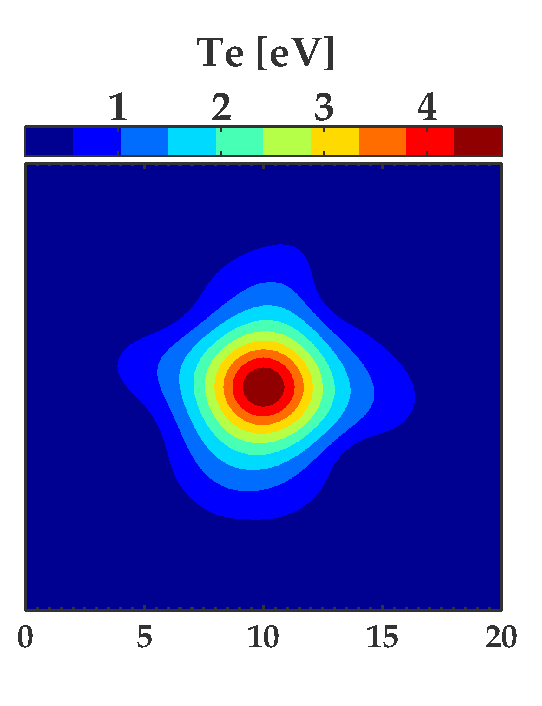
\includegraphics[height=5.5cm]{figures/4-CybeleCarteTemperatureIsolant.eps}}
    \caption{Cartes de densité \subref{4-CybeleCarteDensiteIsolant}~, de
    potentiel \subref{4-CybeleCartePotentielIsolant}~ et de
    température \subref{4-CybeleCarteTemperatureIsolant}}
    \label{CybeleCartesIsolant}
\end{figure}		

A travers cette partie, nous avons tout d'abord vu que 
les solutions calculées par MAGNIS pour une colonne de plasma
sont plutôt cohérentes : Qualitativement, le plasma est confiné dans le plan
transverse et en rotation. La forme caractéristique en spirale, ainsi que
l'intermittence du transport, sont retrouvées. Enfin, et comme le prédit les
théories, l'ajout de parois conductrices dans la direction parallèle (ainsi
que dans la direction perpendiculaire) en permettant de court-circuiter le
plasma, montre la nécessite de tenir compte des pertes en particules et en
courant le long du champ magnétique.

Il est de plus intéressant de préciser que, malgré un maillage cartésien très
peu adapté à la résolution d'un problème cylindrique et l'habituelle difficulté
liée à la discrétisation des flux magnétisés, le schéma de MAGNIS est très
stable, supportant sans difficulté la propagation des discontinuités.

\section{Plasma de bord de tokamaks}

Cette dernière partie est consacrée à la configuration hautement magnétisée
de la SOL, qui correspond à un cas limite de notre étude. Le premier objectif
est toujours de vérifier la validité des solutions calculées par MAGNIS ; 
nous les comparons pour cela avec les résultats de
TOKAM dans sa version isotherme avec conditions aux limites dans la direction
radiale.

\subsection{Un cas critique pour MAGNIS}
Les modèles décrivant les plasmas de SOL ont tous un
point commun :
ils sont construits avec une hypothèse d'ordering basée sur la forte magnétisation des
particules qui permet de simplifier considérablement les équations
du transport transverse dans le plasma, en séparant le mouvement cyclotronique
des mouvements de dérive.
Cette hypothèse d'ordering n'est
toutefois pas applicable dans MAGNIS, l'objectif étant de pouvoir simuler à la
fois les plasmas faiblement et fortement magnétisés. 

La simulation d'un plasma de type SOL avec MAGNIS constitue ainsi un cas idéal
pour :

\begin{itemize}
  \item valider les solutions du transport magnétisé calculées par MAGNIS
  \item	tester le schéma numérique du modèle, dans le cadre d'un plasma
  totalement ionisé et turbulent
  
 \end{itemize} 
\begin{figure}[!htbp]
\centering
\includegraphics[width=0.5\textwidth]{figures/4-tokamSimDomain.png}
\caption{Le domaine de simulation est identique à celui présenté au
chapitre II. La boîte correspond à une petite région de la SOL, de dimension
2cm x 2cm, simulant le côté HFS à gauche de la source et le côté LFS à droite.
\label{4-tokamSimDomain}}
\end{figure}


Nous reprenons les paramètres de simulation utilisés dans le chapitre 2 : Le
champ magnétique, à peu près égal à 1T, est choisi linéairement
décroissant, et correspond à un coefficient de courbure des lignes de champ
g=5.10$^{-4}$.
Le plasma est considéré isotherme et la densité de neutre égale à zéro. La
taille de la zone simulée, dont on rappelle la géométrie
figure~\ref{4-tokamSimDomain}, est de 200 $\rho_\text{L}^i$ soit à peu près
2cm pour une température électronique de 1eV. La longueur de la boîte dans la direction
du champ magnétique est choisie égale à 10m pour obtenir une conductivité
parallèle $\sigma$=10$^{-5}$.

\begin{figure}[!htbp]
  \centering
    \subfigure[]{\label{4-Tokam1}
    \includegraphics[height=8cm]{figures/4-Tokam1.eps}}
    \subfigure[]{\label{4-Tokam2}
    \includegraphics[height=8cm]{figures/4-Tokam2.eps}}
    \caption{Carte de densité telle que calculée par MAGNIS~\subref{4-Tokam1}~
et par TOKAM~\subref{4-Tokam2}~. La densité calculée par TOKAM est ici
redimensionnée avec $n_0~\simeq$~10$^{19}$~m$^{-3}$.}
    \label{4-TokamDensite}
\end{figure}


La figure~\ref{4-TokamDensite} présente les cartes de densité
calculées par MAGNIS et par TOKAM pour ces conditions. On peut
constater que MAGNIS donne des résultats remarquablement proches de ceux
escomptés au vu de la disparité de conception entre les deux modèles. Tout
d'abord, il arrive à capturer le mécanisme de l'instabilité d'interchange , stable quand
$\nabla B\cdot\nabla n<0$ et donnant naissance à un transport intermittent de
type avalanche côté HFS. Le mouvement cyclotronique, que l'on devine au début
des simulations de MAGNIS, se confond très vite dans le transport
macroscopique transverse. Les particules sont enfin principalement
advectées dans la direction radiale entre les structures de potentiel qui se
forment. Ces résultats valident a posteriori l'approximation des vitesses de
dérive, mais montre surtout que MAGNIS donne des solutions correctes
dans des cas fortement magnétisés.

Une différence notable concerne cependant le gradient moyen de potentiel qui
apparaît dans la direction radiale et sur les bords de la simulation\footnote{Plutôt choisies de façon arbitraire dans la simulation de
TOKAM, avec les parois prises totalement absorbantes pour la densité et
fixées au potentiel flottant pour le potentiel, les conditions aux limites
implémentées dans MAGNIS reposent sur un modèle de gaine.}. Cette
tendance donne naissance à
une dérive poloïdale, et se retrouve dans la version anisotherme de TOKAM.
Quand le gradient de densité varie, cette dérive entraîne une diminution du transport transverse à travers un effet de
cisaillement. 

\subsection{Comparaison des profils et de la statistique}

Moyennés dans le temps et sur la direction poloïdale, les profils de densité
(fig.~\ref{4-TokamProfileDensite}) et de flux radial moyen
(fig.~\ref{4-TokamProfileFluxRadial}) sont très proches : sur le profil de
densité, les différences sont possiblement dues aux conditions aux limites
perpendiculaires et parallèle. Le seul écart observable sur le flux radial
moyen (calculé en multipliant le profil moyen de densité par la vitesse
radiale moyenne) se situe à gauche de la source, où la densité est contrôlée par
l'équilibre entre le flux radial diffusif et les pertes le long des lignes de
champ magnétique.

\begin{figure}[!htbp]
  \centering
    \subfigure[]{\label{4-TokamProfileDensite}
    \includegraphics[height=5.5cm]{figures/4-TokamProfileDensite.eps}}
    \subfigure[]{\label{4-TokamProfileFluxRadial}
    \includegraphics[height=5.5cm]{figures/4-TokamProfileFluxRadial.eps}}
    \caption{Comparaison des profils de
    densité~\subref{4-pegasesCompPressTempProfile}~ et de flux
    radial~\subref{4-pegasesCompPressTempProfile}~ entre TOKAM et MAGNIS}
    \label{4-TokamProfils}
\end{figure}

Enfin, la figure~\ref{4-TokamPDFDensite} montre les densités de probabilité des
fluctuations de densité et de flux radial au niveau de la source de particule.
On retrouve là encore un accord très correct, avec une légère déformation de la
PDF, donnant une probabilité plus grande de faible flux dirigé vers les x
décroissant et des évènements (les avalanches) plus importants en sens opposé.

 \begin{figure}[!htbp]
\centering
\includegraphics[width=0.5\textwidth]{figures/4-TokamPDFDensite.eps}
{\caption{Comparaisons des densités de probabilité pour la densité et
le flux radial.}
\label{4-TokamPDFDensite}}
\end{figure}

TOKAM, dont le modèle a été spécifiquement développé pour étudier les plasmas de
SOL, a été validé analytiquement et est encore utilisé quotidiennement dans le
cadre de la recherche sur les plasmas de fusion. La capacité à
reproduire avec autant de similitude ces résultats est très encourageante,
et prouve que MAGNIS peut capturer la physique de base du
transport fortement magnétisé, tout en restant suffisamment stable confronté à un
problème de type turbulent.
Une comparaison instructive pourrait être étudiée prochainement en ajoutant une
densité de neutre et la température électronique.

\end{refsection}
